\documentclass[class=report, crop=false, a4paper, 12pt]{standalone}

%Packages import
\usepackage{../pkgs}


\begin{document}
% A face recognition system works in either or both of two modalities: face verification (or authentication) or face identification (or recognition). The difference between them lies in the final stage of the workflow, identification involves a one-to-one pairing, while identification is a one-to-many match.

\section{Face Recognition - Theory Background}
Face Recognition is a thoroughly debated and extensively researched task in the Computer Vision community for more than two decades~\autocite{ranjanDeepLearningUnderstanding2018}, popularized in the early 1990s with the introduction of the Eigenfaces~\autocite{turkEigenfacesRecognition1991} or Fisherfaces~\autocite{p.n.belhumeurEigenfacesVsFisherfaces1997} approaches. These methods project faces in a low-dimensional subspace assuming certain distributions, but lack the ability to handle uncontrolled facial changes that breaks said assumptions. Henceforth, bringing about face recognition approaches through local-features~\autocite{chengjunliuGaborFeatureBased2002, ahonenFaceDescriptionLocal2006} that, even though, presented considerable results, were not distinctive or compact. Beginning in 2010, methods based on learnable filters have risen~\autocite{z.caoFaceRecognitionLearningbased2010,leiLearningDiscriminantFace2014}, but revealed limitations when nonlinear variations are at stake.

\par Earlier methods for FR worked appropriately when the data was handpicked or generated on a constrained environment. However, they did not scale adequately in the real world were there are large fluctuations in, particularly, pose, age, illumination, background scenario, the presence of facial occlusion~\autocite{ranjanDeepLearningUnderstanding2018} and many unimaginable more~\autocite{kalkaIJBIARPAJanus2018}. These shortcomings can be dealt with by using Deep Learning, a framework of techniques that solves the nonlinear inseparable classes problem~\autocite{minsky69perceptrons}, more specifically a structure called Convolutional Neural Network~\autocite{wangDeepFaceRecognition2021}. 

\par CNNs are a type of Artificial Neural Network that exhibits an improved performance on image or video-based tasks compared to other methods~\autocite{lecunGradientBasedLearningApplied1998}. They were greatly hailed in 2012, after the AlexNet~\autocite{krizhevskyImageNetClassificationDeep2012} victory, by a great margin, in the ImageNet Large Scale Visual Recognition Challenge (ILSVRC). Just two years later, DeepFace~\autocite{taigmanDeepFaceClosingGap2014} revolutionized the benchmarks scores by achieving state-of-the-art results that approached human performance, reinforcing even further the importance of Deep Learning and shifting the research path to be taken~\autocite{wangDeepFaceRecognition2021}.

\par Given what has been stated so far and the proven robustness, performance, and overall results in computer vision, the methods discussed in this dissertation will therefore deal exclusively with Deep Learning approaches. For more information on other methods, please refer to~\autocite{learned-millerLabeledFacesWild2016}. 

\subsection{Convolutional Neural Networks}
\begin{figure}[!h]
    \centering
    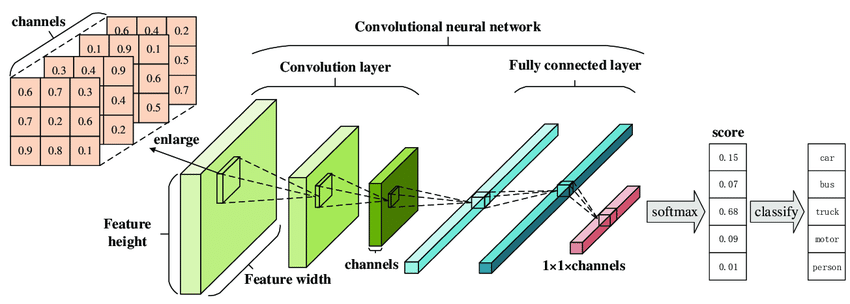
\includegraphics[width=0.85\textwidth]{Architecture-of-a-Convolutional-Neural-Network-CNN-The-traditional-CNN-structure-is.png}
    \caption{Architecture of a Convolutional Neural Network~\autocite{kangDeepSimilarityMetric2019}.}
    \label{fig:cnn}
\end{figure}


\par There are several types of Neural Networks architectures, but CNNs are probably the most widely implemented model overall~\autocite{yamashitaConvolutionalNeuralNetworks2018, liSurveyConvolutionalNeural2022}. Using CNNs for Computer Vision tasks~\autocite{krizhevskyImageNetClassificationDeep2012,taigmanDeepFaceClosingGap2014,tompsonEfficientObjectLocalization2015, zhangImprovedBreastCancer2021}, in this specific case, Face Recognition, is not an arbitrary choice, but due to the fact that the network design benefits from the intrinsic characteristics of the input data: images have an array-like structure~\autocite{yamashitaConvolutionalNeuralNetworks2018}, and local groups of values are correlated (motifs or patterns) and invariant to spatial location~\autocite{lecunDeepLearning2015,caoReviewNeuralNetworks2018}. Furthermore, when compared to fully connected networks, CNNs are superior due to 4 key features: 1) shared weights between the same features in different locations reduce the number of parameters~\autocite{liSurveyConvolutionalNeural2022}, 2) sparse connections~\autocite{alzubaidiReviewDeepLearning2021}, 3) pooling layers and 4) automatically identifies the relevant features without any human supervision~\autocite{alzubaidiReviewDeepLearning2021,liSurveyConvolutionalNeural2022}.

\par In the CNN category itself there are different variants, but they all abide the fundamental structure of a feedforward hierarchical multi-layer network \reffig{fig:cnn}. Feedforward because the information only flows in a singular direction without cycling~\autocite{zellSimulationNeuronalerNetze1994}, hierarchical because the higher complexity internal representations are learned from lower ones~\autocite{lecunDeepLearning2015, zhuBCNNBranchConvolutional2017} and multi-layer because it is composed of a series of stages, blocks or layers. The raw data is fed to an input layer, forwarded to a sequence of intercalating convolutional and pooling layers, transmitted to a stage of one or more fully-connected layers~\autocite{lecunDeepLearning2015, guRecentAdvancesConvolutional2018, alzubaidiReviewDeepLearning2021}.   

\subsubsection{Convolutional Layer}
\par The convolutional layer aims at extracting feature representations from the inputs, and is formed by a set of learnable filters called kernels and an activation function~\autocite{guRecentAdvancesConvolutional2018,yamashitaConvolutionalNeuralNetworks2018}. 

\begin{figure}[!h]
    \centering
    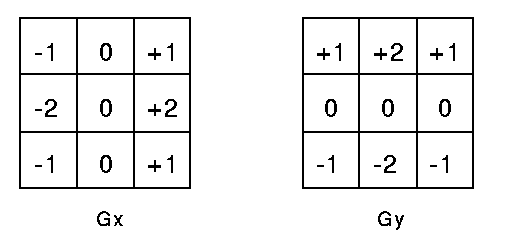
\includegraphics[width=0.45\textwidth]{sobel.png}
    \caption{3x3 Kernels of the Sobel-Feldman operator used for edge detection~\autocite{sobelIsotropicGradientOperator1973}.}
    \label{fig:sobel}
\end{figure}

A kernel \reffig{fig:sobel}, is a grid-like structure of fixed dimensions [WxHxD], where W is the width, H is the height and D is the depth (number of channels). Each of its elements is a learnable weight that is adjusted during training to extract significant features~\autocite{alzubaidiReviewDeepLearning2021}. With a predetermined stride, the kernel scans its receptive field~\autocite{khanSurveyRecentArchitectures2020}, horizontally and vertically, through the input data, and produces the feature map~\autocite{lecunDeepLearning2015, alzubaidiReviewDeepLearning2021} by performing an element-wise product, called convolution, that can be described as follows~\autocite{khanSurveyRecentArchitectures2020}:
\begin{equation}
    f_l^k(p, q) = \sum_{c}^{}\sum_{x, y}^{}i_c(x, y)\cdot w^k_l(u,v)
\end{equation}

where $f_l^k(p, q)$ is an element at line $p$ and column $q$ in the feature map from the k-th kernel in the l-th layer, $i_c(x, y)$ is the element at line $x$ and row $y$ in the input data, and $w^k_l(u,v)$ is the weight at line $u$ and column $v$ from the k-th kernel of the l-th layer.

\begin{figure}[H]
    \centering
    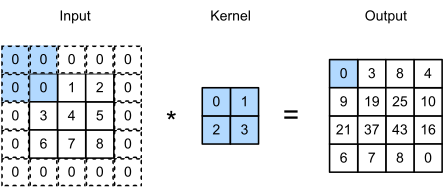
\includegraphics[width=0.6\textwidth]{padding.png} %source: https://d2l.ai/chapter_convolutional-neural-networks/padding-and-strides.html
    \caption{Convolution operation using a $2\times2$ kernel.}
    \label{fig:padding}
\end{figure}

\par The overall architecture of CNNs are inspired by the visual perception~\autocite{hubelReceptiveFieldsBinocular1962}, so a direct parallelism can be made to better define the activation function. The kernels can be seen as receptors, or artificial neurons, that respond to different features, whereas the activation function is a simulation of the threshold function that dictates if the next neuron is activated or not. Additionally, the convolution operation is linear, consequently, if no nonlinear activation function was used, the input of the next layer would be a linear output of the previous layer. The introduction of nonlinearity through activation functions, such as ReLU (Rectified Linear Unit) and its variations (Leaky, Parametric, Randomized, Concatenated, Bounded, etc) or others like Sigmoid or Tanh \autocite{dubeyActivationFunctionsDeep2022}, allows deep neural networks to approximate any function, enhancing the ability to fit to any data~\autocite{liSurveyConvolutionalNeural2022}.

\subsubsection{Pooling Layer}
After the features are extracted, their spatial location becomes less relevant for the following layers. Introducing a pooling layer that reduces the spatial size of the feature maps by joining identical features~\autocite{lecunDeepLearning2015, guRecentAdvancesConvolutional2018}, keeps only the dominant information. This downsampling operation has two important advantages that help reduce the overfitting problem~\autocite{ajitReviewConvolutionalNeural2020,liSurveyConvolutionalNeural2022}. First, it reduces the number of learnable features, which requires less memory to train the network. Second, it enhances feature extraction invariance to shifts and rotations by emphasizing only the relevant features.

\begin{figure}[!h]
    \centering
    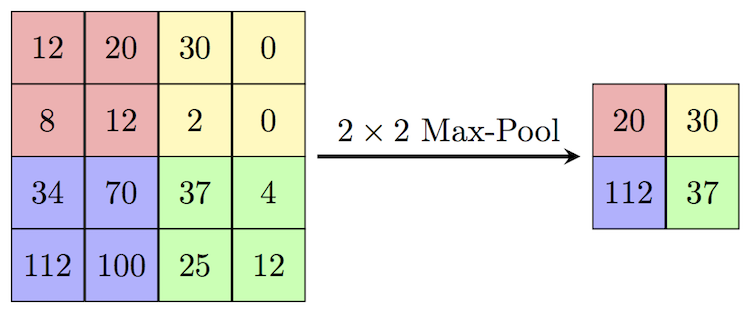
\includegraphics[width=0.6\textwidth]{maxpool.png} %source: https://paperswithcode.com/method/max-pooling
    \caption{Max pool, an example of a pooling operation.}
    \label{fig:maxpool}
\end{figure}

There are many ways of downsampling the feature map through pooling such as min pooling, average pooling or stochastic pooling. However max pooling is by far the most popular one. As pictured in \reffig{fig:maxpool}, this operation divides the feature map in sections and computes the maximum value in each while discarding the other ones.

\subsubsection{Fully Connected Layer}
The fully connected (FC) layer is located at the end of the network. It is a dense, feedforward neural network in which every neuron is connected to all other neurons~\autocite{yamashitaConvolutionalNeuralNetworks2018, alzubaidiReviewDeepLearning2021}. The final feature map is flattened and transformed in a one-dimensional feature vector and the purpose of the FC layer is using this vector as an input, and act as the CNN classifier by performing high logic reasoning~\autocite{guRecentAdvancesConvolutional2018}.

\subsection{Training}
Training a network in the context of CNNs is the process of finding the optimal kernel weights' values. The training data is passed through the model, the predictions asserted and the distance between them and the expected ones is measured by a loss function. LeCun \textit{et al.}~\autocite{lecunGradientBasedLearningApplied1998} presents the problem as follows:
\begin{equation}
    E^p = \mathcal{D}(D^p, Y^p)
\end{equation}

\noindent The loss function, $E^p$, is a measure of error. It computes the difference between the expected result, $D^p$, and the predicted result $Y^p$, where $Y^p = F(Z^p, W)$ is a function of the $p$-th training example, $Z^p$, for a determined weight $W$. Additionally, $E_{train}(W)$, is the average of all the errors calculated in a training set $\left\{(Z^x, D^x),\dots (Z^p, D^p)\right\}$. Training the network is nothing more than a function minimization problem, and for that there are several techniques, the optimizers.

\subsubsection{Optimizers}

% \begin{figure}[H]
%     \centering
%     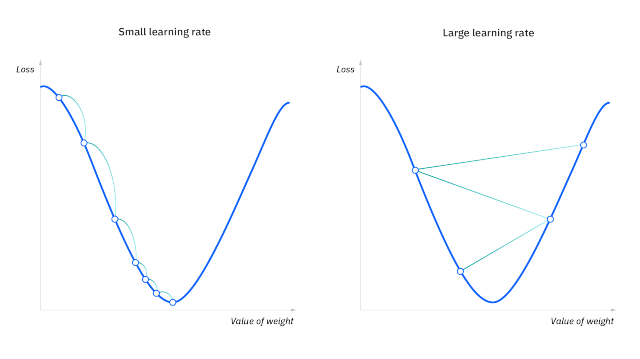
\includegraphics[width=0.6\textwidth]{gd.png} %source: https://www.ibm.com/topics/gradient-descent
%     \caption{Gradient descent}
%     \label{fig:gd}
% \end{figure}


\par By computing the gradient of the loss function in respect to the learnable parameters it allows studying how said parameters influence the loss function and how it can be more efficiently minimized. This algorithm is called gradient descent~\autocite{ruderOverviewGradientDescent}, and is the simplest minimization technique. By definition, the gradient of a function is the direction of the steepest ascent, henceforth, the learnable parameters are updated once every epoch in the opposite direction to reduce the error: 
\begin{equation}
    W_k = W_{k-1}-\epsilon\frac{\delta E(W)}{{\delta} W}
\end{equation}

\noindent where $\epsilon$ is a constant called \textbf{learning rate} that controls how much the parameters are updated and has an immense impact in the performance of a neural network. According to Goodfellow \textit{et al.}~\autocite{Goodfellow-et-al-2016}, if the learning rate is set too low, training will be much slower and can become permanently stuck with a high training error. On the other hand, if the learning rate is too high, the gradient descent can increase the training error instead of reducing it.
\par Stochastic Gradient Descent (SGD)~\autocite{alzubaidiReviewDeepLearning2021} is an efficient algorithm in terms of memory usage, and is the algorithm of choice to optimize the loss function but others such as mini-batch gradient descent or Adam (Adaptive moment estimation)~\autocite{kingmaAdamMethodStochastic2015} are also common.

\subsubsection{Backpropagation}
\par Regardless of the optimizer selected, computing an analytical expression for the gradient is trivial, but evaluating it is a computational heavy task when the aim is to find a minimum with respect to all the parameters in the network. To this extent, the backpropagation algorithm is a solution to do so efficiently~\autocite{6795724} by computing the gradient using an application of the \textit{Chain Rule of Calculus} $\left(\frac{dz}{dx} = \frac{dz}{dy}\frac{dy}{dx}\right)$, that starts at the final layer, and proceeds backwards~\autocite{Goodfellow-et-al-2016}. 

\phantomsection\label{transf learning}
\subsubsection{Transfer Learning} %Source: https://cs231n.github.io/transfer-learning/
\par Developing a Deep Learning system requires data in large scale~\autocite{parkhiDeepFaceRecognition2015}, specially labeled one. In a general sense, gathering information can be very difficult, but if the domain of study is too specific or not widespread enough, that poses an even greater challenge. To overcome this solution, based on the psychologist C.H. Judd's theory, a technique called Transfer Learning takes place. This is defined by Zhuang \textit{et al.}~\autocite{zhuangComprehensiveSurveyTransfer2020} as: given a source and target domain, transfer learning is the act of utilizing the knowledge acquired in the source to further improve the performance of the learned decision functions on the target domain. A classic example is the case of learning how to ride a motorcycle. It will be easier for someone who has already learned how to ride a bicycle than it is to someone starting from scratch.
\par In the context of CNNs, there are 2 ways of approaching the aforesaid problem. By taking a pre-trained CNN and either use it as a fixed feature extractor or fine-tuning it. In the first case, an already trained CNN is used, however, the final few layers or the fully connected one is discarded and retrained to a specific task, while the rest of the network is frozen and used as the feature extractor. The second approach is referred to as fine-tuning a network and, as the name suggests, the source network's parameters are used as a starting point and is retrained using the desired data. That can be achieved by updating the whole network or through freezing the layers. The first ones are the more common since they are responsible for extracting the more general, universal features (edges or patterns).


\newpage
\section{A Face Recognition System}

\begin{figure}[H]
    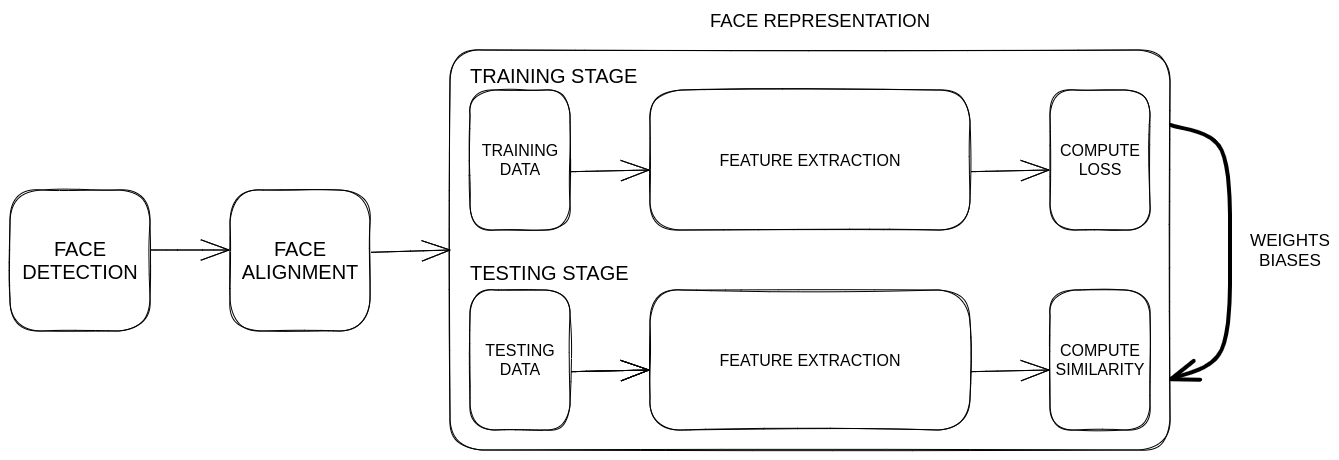
\includegraphics[scale=0.30]{fr_pipeline.png}
    \caption[Pipeline]{A typical learning-based face recognition pipeline, guided by the approach in~\autocite{wangDeepFaceRecognition2021}.}
    \label{fig:fr pipeline}
\end{figure}

\par According to Ranjan \textit{et al.}~\autocite{ranjanDeepLearningUnderstanding2018}, the goal of a face recognition system is to find, process and learn from a face, gathering as much information as possible. As a result, it is one of the most widely implemented biometric system solutions in light of its versatility when facing real world application~\autocite{duElementsEndtoendDeep2022}.

\par All end-to-end automatic face recognition systems follow a sequential and modular\footnote{Sequential because each stage relies on the output from the previous ones, and modular in the sense that each stage employs its own method which can be modified or shapped to better adapt to specific tasks.} pipeline \reffig{fig:fr pipeline} composed of three pillar stages~\autocite{wangDeepFaceRecognition2021}: face detection, face alignment and face representation. First an image or frame from a video is used as an input then, as the name suggests, the \textbf{face detection} module is responsible for finding a face. Next, the \textbf{face alignment} phase applies spatial transformations to the data in order to normalize the faces' pictures to a standardized view. Finally, the \textbf{face representation} stage, makes use of deep learning techniques to learn and further extract discriminative features that will allow the recognition \textit{per se}. A feature is nothing more than a characteristic inherent to the input image that has been measured or processed, and presented as a result~\autocite{Goodfellow-et-al-2016}.

\par All three stages have their individual importance and methods of implementation. \textbf{Face detection} is achievable through classical approaches~\autocite{violaRapidObjectDetection2001, brubakerDesignCascadesBoosted2008} or deep methods, among them is RetinaFace~\autocite{dengRetinaFaceSinglestageDense2019} and MTCNN~\autocite{zhangJointFaceDetection2016a}. \textbf{Face alignment}, once again, can be accomplished through traditional measures~\autocite{cootesViewbasedActiveAppearance2002, martinezLocalEvidenceAggregation2013} or more modern ones, namely PropagationNet~\autocite{huangPropagationNetPropagatePoints2020} or, yet again, MTCNN~\autocite{zhangJointFaceDetection2016a} which concurrently performs detection and alignment. To conclude, the \textbf{face representation} module is no exception, and can also be divided in two groups, regarding the methodology used. Some conventional systems were already mentioned, such as Eigenfaces~\autocite{p.n.belhumeurEigenfacesVsFisherfaces1997,turkEigenfacesRecognition1991}, and the deep learning ones are the object of discussion of this dissertation and will be reviewed along the following sections. As such, the focus will be on describing, with particular interest, the face representation stage. For a deeper and extensive study, please refer to:~\autocite{zafeiriouSurveyFaceDetection2015} in the case of classic face detection approaches and~\autocite{minaeeGoingDeeperFace2021} for deep learning based methods;~\autocite{wangFacialFeaturePoint2018} addresses traditional face alignment methods and is complemented with~\autocite{duElementsEndtoendDeep2022} for more up-to-date techniques; and~\autocite{learned-millerLabeledFacesWild2016} tackles classic face representation.

\subsection{Face Detection}
\par Face detection is the first step in any automatic facial recognition system. Given an input image to a face detector module, it is in charge of detecting every face in the picture and returning bounding-boxes coordinates, for each one, with a certain confidence score~\autocite{duElementsEndtoendDeep2022,ranjanDeepLearningUnderstanding2018}.

\par Previously employed traditional face detectors are incapable of detecting facial information when faced with challenges such as variants in image resolution, age, pose, illumination, race, occlusions or accessories (masks, glasses, makeup)~\autocite{duElementsEndtoendDeep2022,ranjanDeepLearningUnderstanding2018}. The progress in deep learning and increasing GPU power led Deep CNNs (DCNNs) to become a viable and reliable option that solves said problems in face detection. Methods such as CenterFace~\autocite{xuCenterFaceJointFace2019}, MTCNN~\autocite{zhangJointFaceDetection2016a} or RetinaFace\autocite{dengRetinaFaceSinglestageDense2019} are examples of the more commonly adopted state-of-the-art approaches.

\par These techniques can be included in different categories depending on the method's characteristics. A more analytical perspective~\autocite{duElementsEndtoendDeep2022} distributes the methods, depending upon their architecture or purpose of application, over seven categories: multi-stage, single-stage, anchor-based, anchor-free, multi-task learning, CPU real-time and, finally, problem-oriented. To an in depth review of each category, refer to the \hyperref[sec:face_detection_appendix]{Appendix}.

\vspace{0.5\baselineskip}
\begin{figure}[h!]
    \centering
    \begin{minipage}[c]{0.38\textwidth}
      \centering
      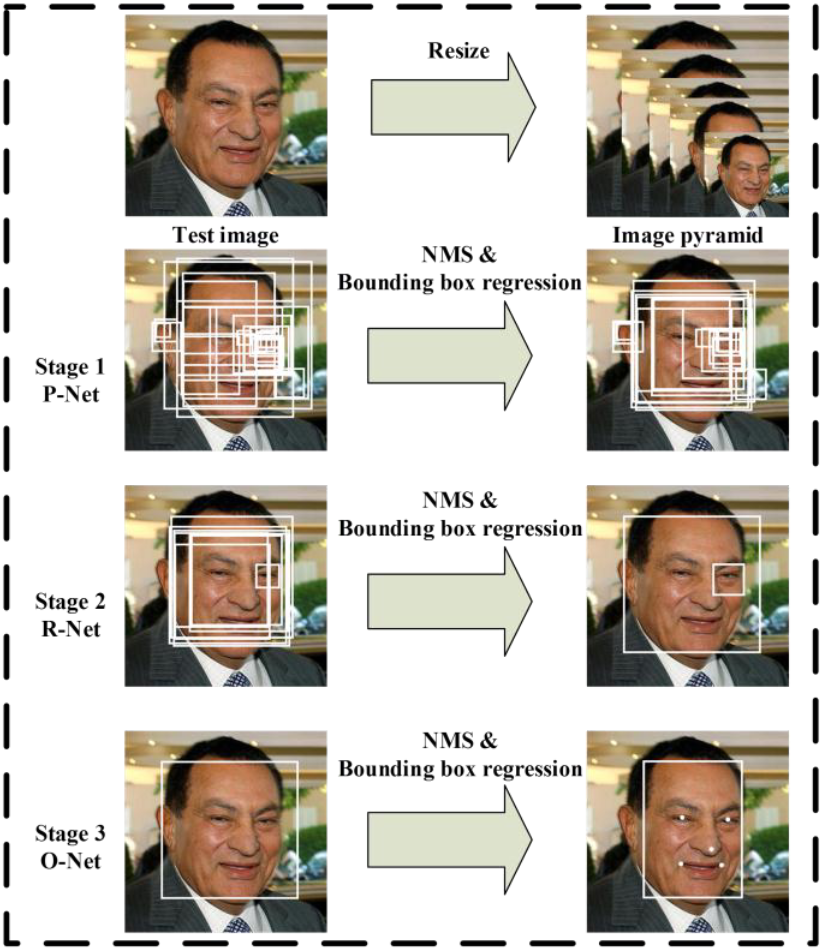
\includegraphics[width=\textwidth]{mtcnn.png}
      \label{fig:mtcnn}
    \end{minipage}
    \hspace{0.5cm}
    \begin{minipage}[c]{0.52\textwidth}
      \centering
      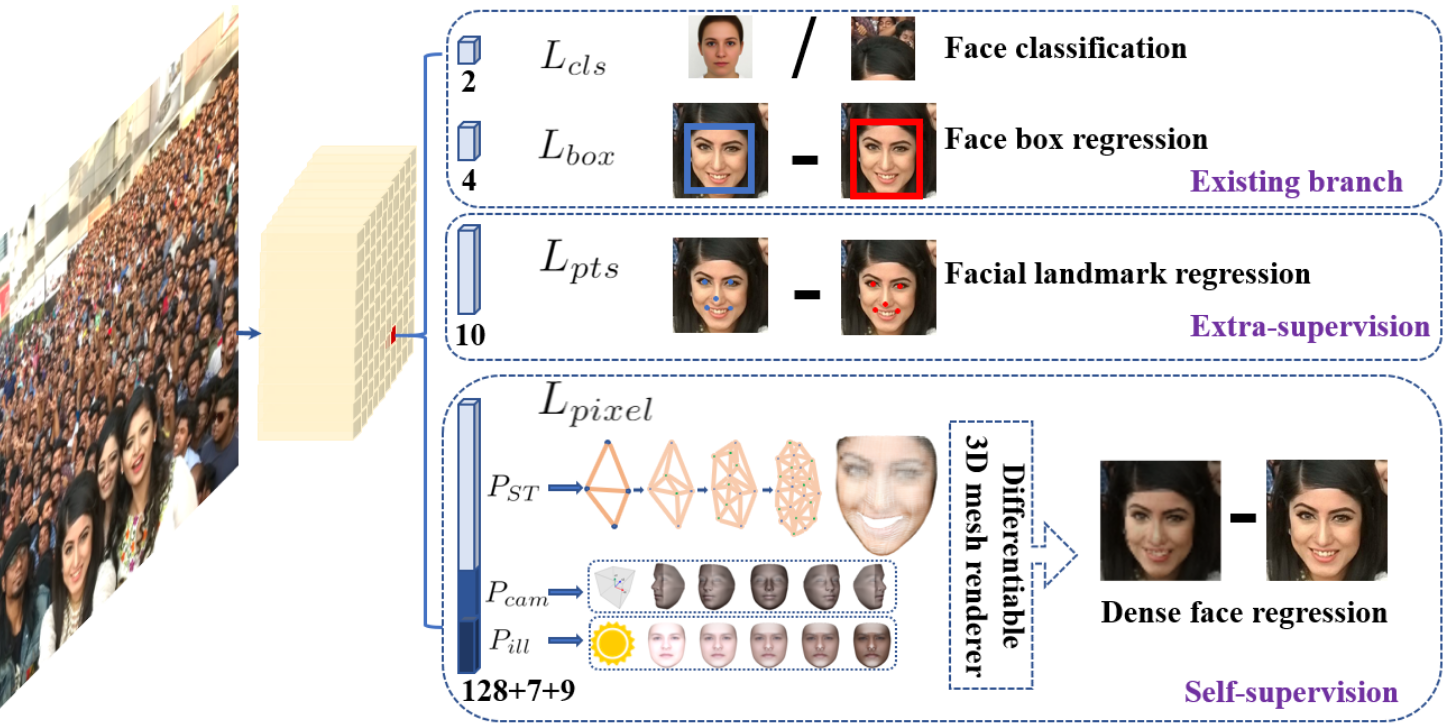
\includegraphics[width=\textwidth]{retinaface.png}
      \label{fig:retinaface}
    \end{minipage} 
    \begin{minipage}{0.4\textwidth}
        \vspace{-0.5cm}
        \centering
        \footnotesize a)
    \end{minipage}
    \hfill
    \begin{minipage}{0.4\textwidth}
        \vspace{-0.5cm}
        \centering
        \footnotesize b)
    \end{minipage}
    \vspace{-0.4cm}
    \caption{Comparison between \textbf{a)} MTCNN: multi-stage, CPU real-time and multi-task learning, and \textbf{b)} RetinaFace: single-stage, anchor-based, CPU real-time and multi-task learning. MTCNN~\autocite{zhangJointFaceDetection2016a} proposes a series of bounding boxes then, through a series of refinement stages, the best solution and landmarks are found. RetinaFace~\autocite{dengRetinaFaceSinglestageDense2019} accomplishes, in a single-stage, face classification and bounding box regression by evaluating anchors, landmark localization and dense 3D projection for facial correspondence.}
    \label{fig:mtcnn vs retinaface}
\end{figure}


\subsection{Face Alignment}
\par Face Alignment, or facial landmark detection~\autocite{changFacePoseNetMakingCase2017}, is the second stage of the face recognition pipeline, and has the objective of calibrating the detected face to a canonical layout, through landmark-based or landmark-free approaches, in order to leverage the core final stage of face representation~\autocite{duElementsEndtoendDeep2022}. 
\par Despite the fact that traditional face alignment methods are very accurate, that only occurs in constrained circumstances. Therefore, once again, to address that issue, deep learning-based methods are the solution to perform an accurate facial landmark localization that realistically scales to real world scenarios~\autocite{fengWingLossRobust2018}. 
\par Furthermore, face alignment, can be accomplished through two categories of methods: landmark-based and landmark-free. Landmark-based alignment leverages facial landmarks (eyes, mouth, nose, etc.) to normalize the image to a layout through spatial transformations~\autocite{duElementsEndtoendDeep2022}. Methods like Wing loss~\autocite{fengWingLossRobust2018}, Kernel Density Deep Neural Network~\autocite{chenFaceAlignmentKernel2019} or the Recurrent Dual Refinement (RDR) proposed in~\autocite{xiaoRecurrent3D2DDual2017} integrate this category. Landmark-free alignment, as the name obviously suggests, is the category of methods that align the face without points of reference, namely RDCFace~\autocite{zhaoRDCFaceRadialDistortion2020} or the one proposed by by Hayat \textit{et al.}~\autocite{hayatJointRegistrationRepresentation2017}. The \hyperref[sec:face_alignment_appendix]{Appendix} presents more details regarding the aforementioned.

\vspace{0.7\baselineskip}
\par As can be seen from the previous section, this step in the face recognition process can be accomplished, very sporadically, through standalone methods that process the detected face from the previous stage, but generally joint detection and alignment methods, such as RetinaFace \autocite{dengRetinaFaceSinglestageDense2019}, are the optimal choice~\autocite{changFacePoseNetMakingCase2017}.

\subsection{Face Representation}
\par Finally, Face Representation is the last stage of the Face Recognition process. It is responsible for processing the aligned face from the previous stage and mapping the produced feature representation to a feature space, in which features from the same person are closer together and those that are different stand further apart from each other~\autocite{duElementsEndtoendDeep2022}.
\par According to the literature~\autocite{duElementsEndtoendDeep2022,liHandbookFaceRecognition2011,ranjanDeepLearningUnderstanding2018,schroffFaceNetUnifiedEmbedding2015,wangDeepFaceRecognition2021}, there is a consensus about how Face Recognition can be performed in two settings of operation: face verification and face identification. This distinction is only made possible due to the approaches available in the Face Representation stage that can leverage one, the other or both. Face verification, is a one-to-one, pair-wise match, and it is the action of verifying if the query face matches the identity that is being claimed. These principles are used in biometric systems such as self-service immigration clearance using E-passport~\autocite{liHandbookFaceRecognition2011}. Face identification, is a one-to-many correlation process that compares a query face to a database of faces and associates it to the corresponding match (or matches). A typical use case is to identify someone in a watchlist or surveillance videos~\autocite{liHandbookFaceRecognition2011}.



\vspace{0.7\baselineskip}
\par The overall pipeline comes to a conclusion in this module. However, as can be seen in \reffig{fig:fr pipeline}, due to its importance for the face recognition problem, it is highlighted the inherent pipeline of the Face Representation stage is discussed in depth in the next section.

\section{Face Representation Pipeline}
\begin{figure}[!h]
    \centering
    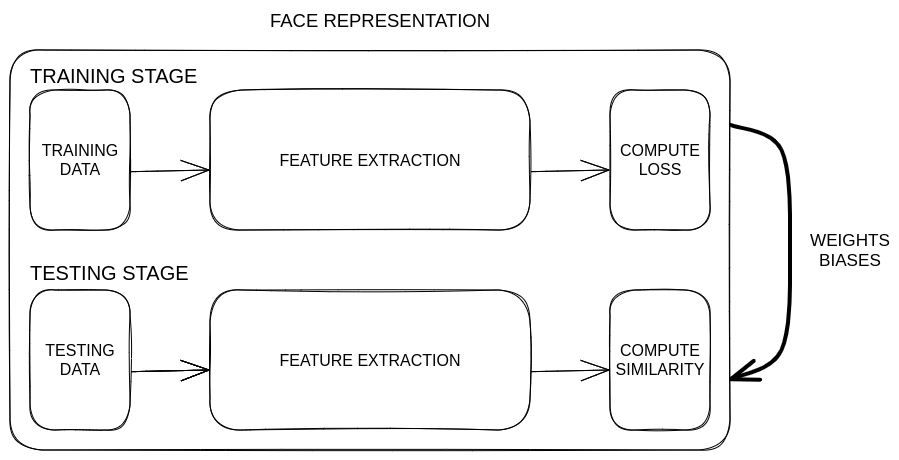
\includegraphics[scale=0.4]{frep_pipeline.png}
    \caption[Pipeline]{Face Representation pipeline, guided by the approach in~\autocite{wangDeepFaceRecognition2021}.}
    \label{fig:frep pipeline}
\end{figure}

\par As show in \reffig{fig:frep pipeline}, Face Representation is a two-step module composed of a training and testing stage. So as to be capable of performing face recognition, in either a verification or identification manner, a face representation system needs to learn robust, invariant and discriminative features that can distinguish identities~\autocite{ranjanDeepLearningUnderstanding2018}. 
\par To meet these requirements, the feature extractor must first be trained properly by taking data from previous stages and outputting a feature representation that is compared to the desired value using a loss function~\autocite{lecunDeepLearning2015, wangDeepFaceRecognition2021}. After that, everything is ready for the testing stage, where the face recognition \textit{per se} occurs by calculating a similarity score for the feature representation produced by the trained feature extractor, and dictating if the identity belongs to the same person (face verification) or if it matches any identity (face identification)~\autocite{ranjanDeepLearningUnderstanding2018}.



\subsection{Datasets: Training and Testing Data}
\par As been discussed throughout this dissertation, Deep Learning techniques can solve the problem of handling unconstrained scenarios, where there are variations in pose, illumination, occlusion, and so forth. To support this, in the past few years, datasets have been developed with this in mind so to be able to provide a large and diverse set of both training data, allowing for adequate regularization to unseen circumstances, and testing data that benchmarks the face recognition system in, as similar as possible, unconstrained real world scenarios~\autocite{duElementsEndtoendDeep2022}. 

\vspace{\baselineskip}
In the following pages, a mix of training datasets, of overall relevance and more geared towards the purpose of this dissertation, will be reviewed.

\subsubsection{\large Training Data}
\par When developing a deep face recognition system it is essential to keep in mind its necessity to adapt, and that is where the dataset used for training comes at play. Large training datasets are essential for face recognition~\autocite{parkhiDeepFaceRecognition2015}, but large-scale is not enough. There must be a balance between the depth (number of unique identities) and the breadth (or width) (number of images per identity)~\autocite{bansalDonTsCNNbased2017, caoVGGFace2DatasetRecognising2018}, and it will lead to different effects. On one hand, a training dataset that is deep will help the face recognition system to produce more discriminative feature representations, since it will have a great number of identities to learn from. On the other hand, a wider set will have more images per identity, therefore, variations in pose, expressions, illuminations, occlusions, background clutter, image quality, accessories, and so forth~\autocite{baeDigiFace1MMillionDigital2023} can be introduced and ultimately lead to more robust feature representations.

% 

\begin{table}[!ht]
    \centering
    \caption{Comparison of the training datasets. \cmark - Datasets that are still available to the public. \xmark  - Datasets that have been removed from distribution.}
    \resizebox{\textwidth}{!}{%
    \begin{tabular}{|l|c|c|c|c|c|c|c|}
    \hline
    \multicolumn{1}{|c|}{\textbf{Dataset}} & \textbf{Year} & \textbf{Availability} & \textbf{Images/videos} & \textbf{Depth} & \textbf{Avg. Breadth} & \textbf{Distribution} & \textbf{Description} \\ \hline
    CASIA-WebFace~\autocite{yiLearningFaceRepresentation2014}                         & 2014          & \xmark          & 494,414/-              & 10,575         & 46.7                  & Public                & First public face recognition dataset.                 \\ \hline
    \textit{Facebook}~\autocite{taigmanWebscaleTrainingFace2015}                               & 2015          & \xmark                     & 500M/-                 & 10M            & 50                    & Private               & \textit{Facebook}'s private dataset used to test different properties in face identification.                 \\ \hline
    \textit{Google}~\autocite{schroffFaceNetUnifiedEmbedding2015}                                 & 2015          & \xmark                     & 200M/-                 & 8M             & 25                    & Private               & Private dataset used to train the FaceNet method.                 \\ \hline
    VGGFace~\autocite{parkhiDeepFaceRecognition2015}                                & 2015          & \xmark          & 2,6M/-                 & 2,622          & 991.6                 & Public                & High width public dataset released alongside VGGFace method.                 \\ \hline
    MS-Celeb-1M~\autocite{guoMSCeleb1MDatasetBenchmark2016}                           & 2016          & \xmark          & 10M/-                  & 100k           & 100                   & Public                & Large-scale celebrities dataset.                 \\ \hline
    MegaFace~\autocite{nechLevelPlayingField2017}                               & 2016          & \xmark                  & 4,753,320/-            & 672,057        & 7.1                   & Public                & Non-celebrity dataset.                 \\ \hline
    VGGFace2~\autocite{caoVGGFace2DatasetRecognising2018}                               & 2017          & \xmark                  & 3,31M/-                & 9131           & 362.5                 & Public                & High characteristics variation dataset.                 \\ \hline
    UMDFaces-Videos~\autocite{bansalDonTsCNNbased2017}                        & 2017          & \xmark                  & -/22,075               & 3,107          & 7.1                   & Public                & Video-based dataset with great variations.                 \\ \hline
    Celeb-500k~\autocite{caoCeleb500KLargeTraining2018}                             & 2018          & \cmark                  & 50M/-                  & 500k           & 100                   & Public                & Noisy celebrities dataset.                 \\ \hline
    Celeb-500k-2R~\autocite{caoCeleb500KLargeTraining2018}                          & 2018          & \cmark                  & 25M/-                  & 245k           & 102                   & Public                & Cleaned version.                 \\ \hline
    IMDb-Face~\autocite{wangDevilFaceRecognition2018}                              & 2018          & \cmark                  & 1,7M/-                 & 59k            & 28.8                  & Public                & Manually cleaned revision of MS-Celeb-1M and MegaFace.                 \\ \hline
    MS1MV2~\autocite{dengArcFaceAdditiveAngular}                                 & 2019          & \cmark                  & 5,8M/-                 & 85k            & 68.2                  & Public                & Semi-automatic cleaned version of MS-Celeb-1M.                 \\ \hline
    RMFRD~\autocite{wangMaskedFaceRecognition2020}                                 & 2020          & \cmark                  & 95k/-                  & 525            & 180.9                 & Public                & Dataset of masked and unmasked celebrities.                 \\ \hline
    Glint360k~\autocite{anPartialFCTraining2021}                              & 2021          & \cmark                  & 17M/-                  & 360k           & 47.2                  & Public                & Cleaned version of the Celeb-500k AND MS1MV2 datasets.                \\ \hline
    WebFace260M~\autocite{zhuWebFace260MBenchmarkUnveiling2021}                            & 2021          & \cmark                  & 260M/-                 & 4M             & 65                    & Public                & Largest publicly available dataset of celebrities faces (noisy).                 \\ \hline
    WebFace42M~\autocite{zhuWebFace260MBenchmarkUnveiling2021}                             & 2021          & \cmark                  & 42M/-                  & 2M             & 21                    & Public                & Cleaned and smaller version.                 \\ \hline
    WebFace4M~\autocite{zhuWebFace260MBenchmarkUnveiling2021}                              & 2021          & \cmark                  & 4,2M/-                 & 200k           & 21                    & Public                & Smaller version.                 \\ \hline
    DigiFace-1M~\autocite{baeDigiFace1MMillionDigital2023}                            & 2022          & \cmark                  & 1,22M/-                & 110k           & 11.1                  & Public                & Large-scale, fully synthetic dataset.                 \\ \hline
    \end{tabular}%
    }
    
    \label{tab:training data}
\end{table}

\par \autoref{tab:training data} showcases large scale datasets that are the usual source of training data. Some noteworthy examples: CASIA-WebFace~\autocite{yiLearningFaceRepresentation2014} that was the first public one of this kind; MS-Celeb-1M~\autocite{guoMSCeleb1MDatasetBenchmark2016} that gathers 10 million images from 100 thousand celebrities; MS1MV2~\autocite{dengArcFaceAdditiveAngular}, the semi-automatic cleaned version of MS-Celeb-1M; MegaFace~\autocite{nechLevelPlayingField2017}, which introduces close to 5 million images from 670 thousand non-celebrity identities; WebFace260M~\autocite{zhuWebFace260MBenchmarkUnveiling2021} revolutionizes the dataset space with 260 million faces from 4 million identities; DigiFace-1M~\autocite{baeDigiFace1MMillionDigital2023}, a synthetic dataset that addresses privacy violations, lack of informed consent and exploitation of distribution licenses and vague terms (such as "celebrities") to gather data are some of the criticisms that raised enough concerns that lead to revoking the distribution of several datasets. 

\newpage
\subsubsection{\large Testing Data}

\par After the training is completed the performance of the system needs to be evaluated on different challenges to properly access if it scales (or generalizes) to real-world scenarios. The way of doing so is by employing test datasets, where their evaluation protocols are designed to perform pair matching, that is, face verification. 

\begin{table}[!ht]
    \centering
    \caption{Comparison of the test datasets. \cmark - Datasets that are still available to the public. \xmark - Datasets that have been removed from distribution.}
    \resizebox{\textwidth}{!}{%
    \begin{tabular}{|l|c|c|c|c|c|c|c|}
    \hline
    \multicolumn{1}{|c|}{\textbf{Dataset}} & \textbf{Year} & \textbf{Availability} & \textbf{Images/videos} & \textbf{Depth} & \textbf{Avg. Breadth} & \textbf{Description} \\ \hline
    LFW~\autocite{huangLabeledFacesWild}                                    & 2007          & \xmark          & 13,233/-              & 5,749         & 2.3                  & The most well known face verification public dataset.                 \\ \hline
    YTF~\autocite{wolfFaceRecognitionUnconstrained2011}                                    & 2011          & \cmark                     & -/3,425                 & 1595            & 2.1                    & Face verification video dataset inspired on the LFW                 \\ \hline
    IJB-A~\autocite{klarePushingFrontiersUnconstrained2015}                                  & 2015          & \xmark                     & 5,712/2,085                 & 500             & 11.4/4.2                    & Benchmark that aims at straying from accuracy saturation by proposing a more challenging dataset.                 \\ \hline
    CFP~\autocite{senguptaFrontalProfileFace2016}                                 & 2016          & \xmark          & 7,000/-                 & 500          & 14                 & Studies the effect of extreme pose variations on face verification.                 \\ \hline
    CPLFW~\autocite{zhengCrossPoseLFWDatabase}                                  & 2017          & \cmark                  & 13,233/-            & 5,749        & 2.3                   & Variation of the LFW for different poses with refined verification pairs.                 \\ \hline
    CALFW~\autocite{zhengCrossAgeLFWDatabase2017}                                  & 2017          & \cmark                  & 13,233/-                & 5,749           & 2.3                 & Same principles of CPLFW but applied to age related tests.                 \\ \hline
    AgeDB~\autocite{moschoglouAgeDBFirstManually2017}                                  & 2017          & \cmark                  & 16,488/-               & 568          & 29.0                   & Similar to CALFW but promotes noise free labelling by doing it manually.                 \\ \hline
    IJB-B~\autocite{whitelamIARPAJanusBenchmarkB2017}                                 & 2017          & \xmark                  & 21,798/7,011                  & 1,845           & 11.8/3.8                   & Improvement over the IJB-B dataset (more data and more possible pairs).                 \\ \hline
    TinyFace~\autocite{chengLowResolutionFaceRecognition2019}                               & 2018          & \cmark                  & 15,975 (153,428)/-                  & 5,139           & 3.1                   & Genuine low resolution face recognition benchmark.                 \\ \hline
    IJB-C~\autocite{mazeIARPAJanusBenchmark2018}                                  & 2018          & \xmark                  & 31,334/11,779                 & 3,531            & 8.9/3.3                  & IJB-B refinement (more protocols and increased individuals diversity).                 \\ \hline
    IJB-S~\autocite{kalkaIJBIARPAJanus2018}                                  & 2018          & \xmark                  & 5,656/350 (202)                 & 202            & 28/2.7                  & Very challenging manually annotated benchmark.                 \\ \hline
    RFW~\autocite{wangRacialFacesWild2019}                                    & 2018 & \cmark                  & 40,607/-                  & 11,429            & 3.5                 & Benchmarks the racial bias of face verification methods.                 \\ \hline          
    QMUL-SurvFace~\autocite{chengSurveillanceFaceRecognition2018}                          & 2018          & \cmark                  & 463,507/-                  & 15,573            & Public                & Dataset colected in uncooperative surveillance scenarios, presenting high variance of characteristics.                  \\ \hline
    MDMFR~\autocite{ullahNovelDeepMaskNetModel2022}                                  & 2021          & \cmark                  & 2,896/-                  & 226            & 12.8                 & Large scale dataset for masked face recognition.                 \\ \hline
    XQLFW~\autocite{knocheCrossQualityLFWDatabase2021}                                  & 2021          & \cmark                  & 13,233/-                  & 5,749           & 2.3                  & LFW variation to study the effect of resolution on face verification.                 \\ \hline
    CAFR~\autocite{zhaoAgeInvariantFaceRecognition2022}                                   & 2022          & \cmark                  & 1,446,500/-                  & 25,000            & 57.9                 & Large scale dataset to study the impact of individual's age.                 \\ \hline
    FaVCI2D~\autocite{popescuFaceVerificationChallenging2022}                                & 2022          & \cmark                  & 64,879/-                 & 52,411             & 1.2                    & Face verification dataset that addresses easy pairs, demographic bias and ethical concerns.                 \\ \hline
    \end{tabular}%
    }
    
    \label{tab:test data}
\end{table}

\par One of the most well known test data set is LFW~\autocite{huangLabeledFacesWild}, but with the evolution of face recognition methods, it quickly became saturated in terms of accuracy reports. This motivated investigations to develop more challenging datasets, like A, B, C and S IJB benchmarks~\autocite{klarePushingFrontiersUnconstrained2015, whitelamIARPAJanusBenchmarkB2017, mazeIARPAJanusBenchmark2018, kalkaIJBIARPAJanus2018}, QMUL-SurvFace~\autocite{chengSurveillanceFaceRecognition2018} and YTF (for video tests)~\autocite{wolfFaceRecognitionUnconstrained2011}, or for specific hurdles~\autocite{duElementsEndtoendDeep2022}, for instance, CPLFW~\autocite{zhengCrossPoseLFWDatabase} or CFP~\autocite{senguptaFrontalProfileFace2016} for cross-pose, CALFW~\autocite{zhengCrossAgeLFWDatabase2017} or AgeDB30~\autocite{moschoglouAgeDBFirstManually2017} for cross-age, RFW~\autocite{kalkaIJBIARPAJanus2018} for racial variations, XQLFW~\autocite{knocheCrossQualityLFWDatabase2021} for quality assessment or MDMFR~\autocite{ullahNovelDeepMaskNetModel2022} for masked reocgnition. Although some of the previously referenced datasets do have a benchmarking component and are described as such, they can also be generally employed to train or fine-tune algorithms for specific challenges.
\par For a better description of all the datasets see the \hyperref[sec:train_data_appendix]{Train Data Appendix} and \hyperref[sec:test_data_appendix]{Test Data Appendix}.

\subsection{Feature Extractor}
A feature extractor is present in both the training and testing stage of the Face Representation process, as it allows the visual data to be processed for evaluation by transforming the input into low dimensional representations~\autocite{lecunGradientBasedLearningApplied1998}. It is also what distinguishes a Conventional Machine Learning approach from a Deep Learning one.  
\par The following methods are all based in deep learning, therefore the \textit{modus operandi} abides by the same principles and can be outlined as follows: 1) the feature extractor is a deep neural network, more specifically a Convolutional Neural Network (CNN), that is trained with a loss function, 2) the trained feature extractor contains prior knowledge and is applied on unseen test data and 3) the results are used to compute 1:N similarity (face identification - ``who is this person?'') or 1:1 similarity (face verification - ``are these persons the same?'').
\par Over the years, the architecture of CNNs evolved and became of great importance to all image related tasks. Other than the already mentioned revolutionary AlexNet~\autocite{krizhevskyImageNetClassificationDeep2012}, there are other designs that significantly contributed to breakthroughs and broken benchmark records. There can be general architectures, like VGGNet~\autocite{simonyanVERYDEEPCONVOLUTIONAL2015}, GoogLeNet~\autocite{szegedyGoingDeeperConvolutions2014}, ResNet~\autocite{heDeepResidualLearning2016}, iResNet~\autocite{dutaImprovedResidualNetworks2021}, or specialized architectures. For example, lightweight face recognition implementations such as MobileFaceNet~\autocite{chenMobileFaceNetsEfficientCNNs2018}, VarGFaceNet~\autocite{yanVarGFaceNetEfficientVariable2019}, MixFaceNet~\autocite{boutrosMixFaceNetsExtremelyEfficient2021} and ConvFaceNeXt~\autocite{hooConvFaceNeXtLightweightNetworks2022}.

\vspace{\baselineskip}
\noindent\textbf{$\rightarrow$ VGGNet}~\autocite{simonyanVERYDEEPCONVOLUTIONAL2015} took inspiration from AlexNet and improved its accuracy in image classification by studying the effect of the network's depth. It accomplished that by substituting the 11x11 convolution kernel with stride 4 for a stack of very small 3x3 receptive field with stride 1. The final best performing model was 19 layers deep (16 convolutional and 3 fully-connected) and had 144 million parameters.

\begin{figure}[H]
    \centering
    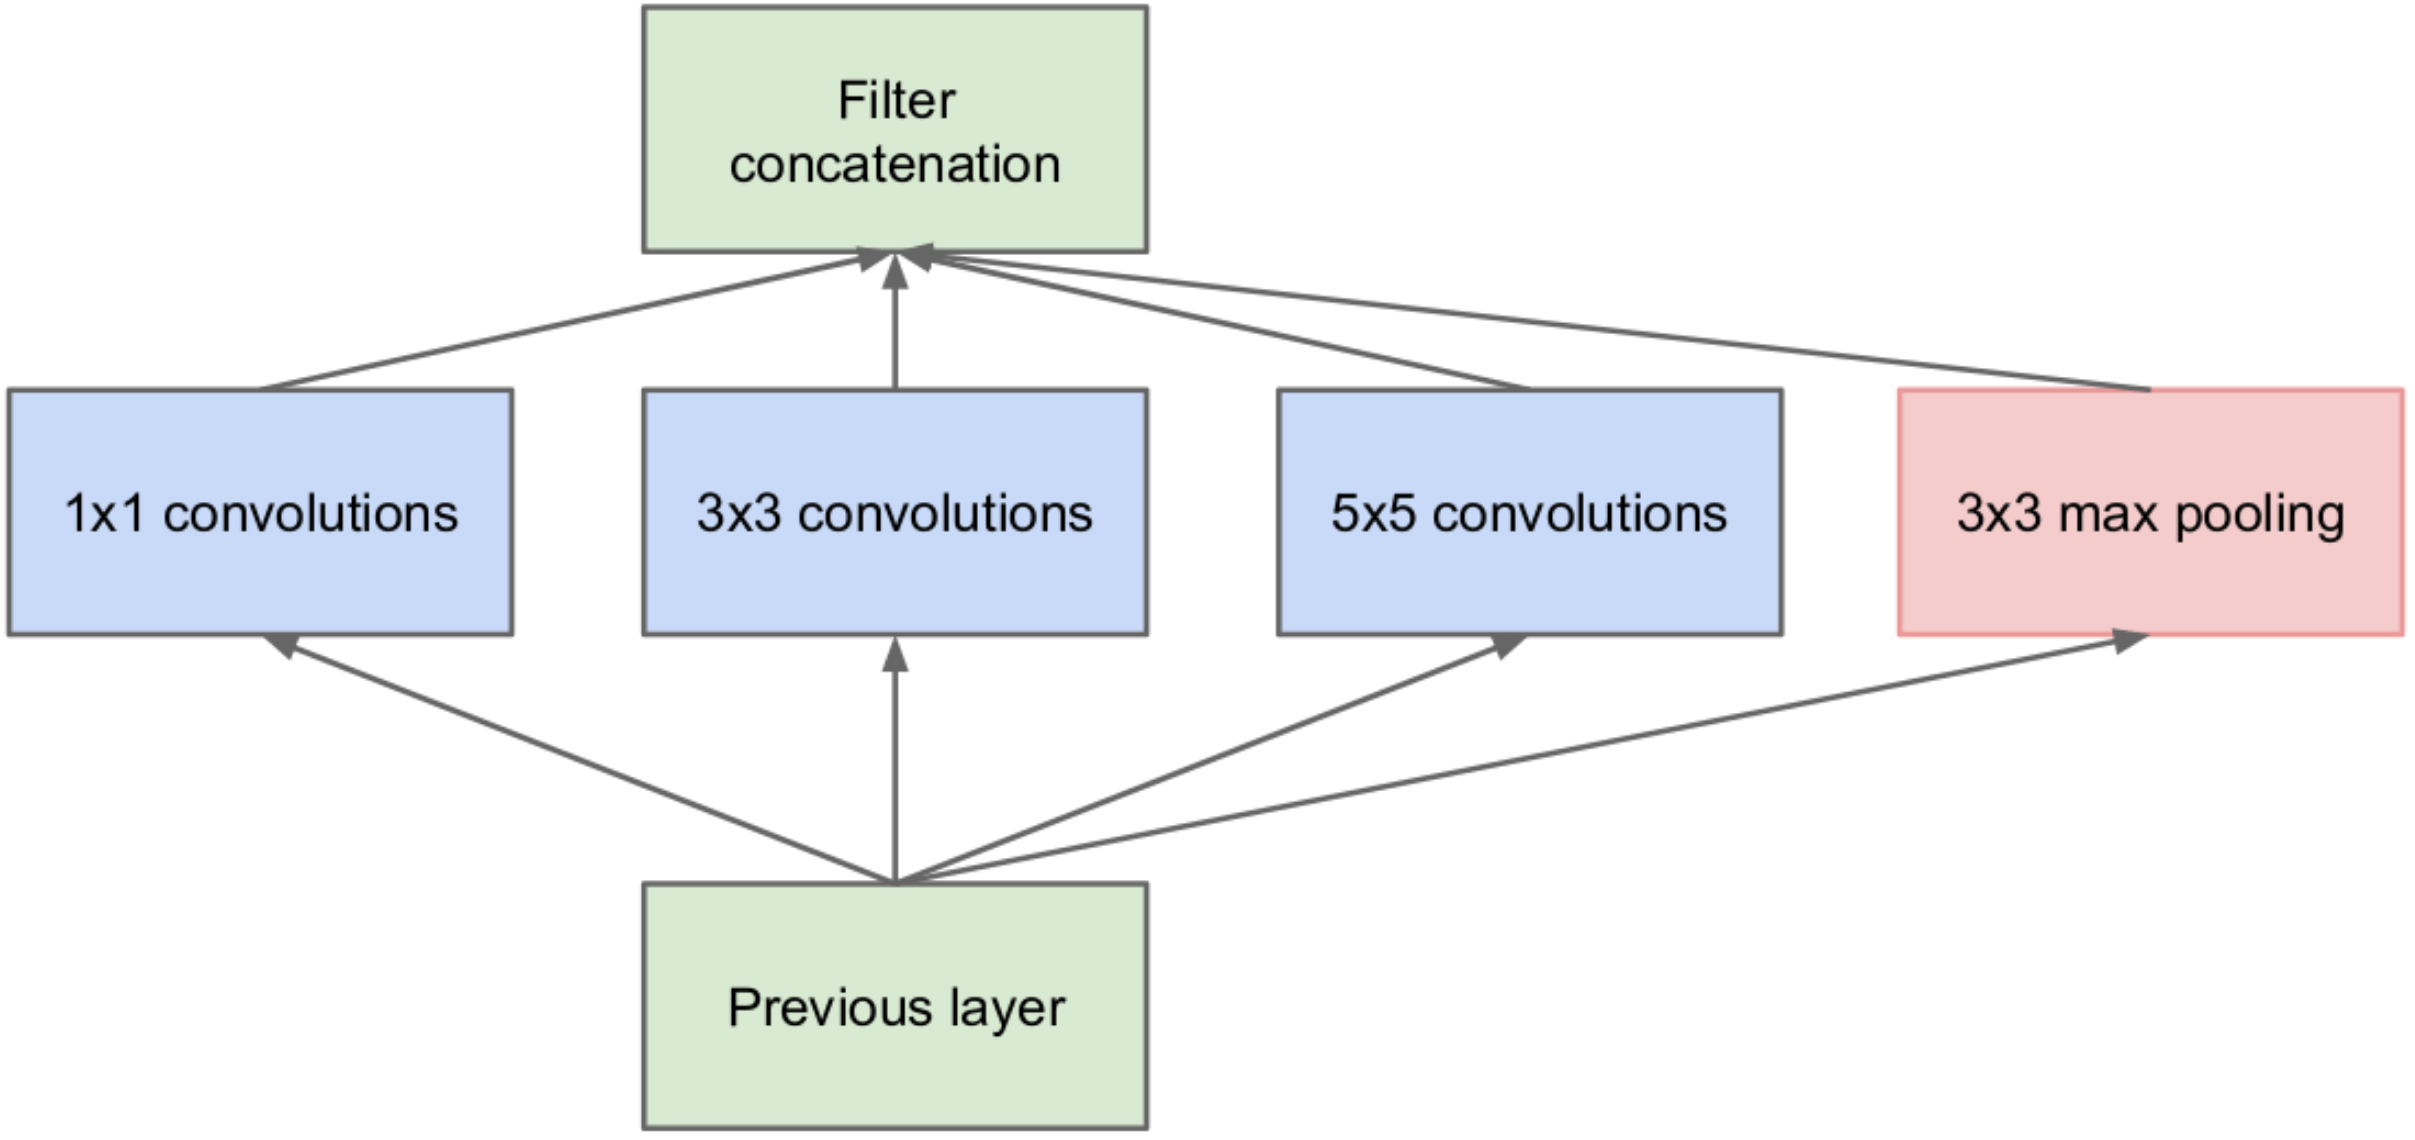
\includegraphics[scale=0.11]{inception_naive.png}
    \caption{GoogLeNet's inception block from the original paper~\autocite{szegedyGoingDeeperConvolutions2014}.}
    \label{fig:inception}
\end{figure}

\noindent\textbf{$\rightarrow$ GoogLeNet}~\autocite{szegedyGoingDeeperConvolutions2014}, also known as Inception-V1, aimed at reducing the computational cost associated with training and employing a network, while retaining highly accurate results. That was accomplished by introducing sparse connectivity (not all feature maps are shared with the forward layers), an inception block \autoref{fig:inception}, consisting of multi-scale convolutional layers with small blocks of different sized kernels (1x1, 3x3 and 5x5), and replacing the last fully connected layer with a global averaging pooling one and adding a dimension lowering bottleneck layer of 1x1 convolution before large kernels. These changes helped to achieve a low number of 4 million parameters (12x fewer than the revolutionary AlexNet and 36x less than VGGNet)

\vspace{0.7\baselineskip}
\begin{figure}[H]
    \centering
    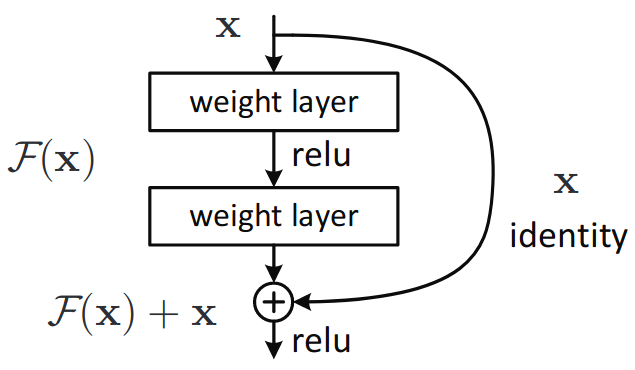
\includegraphics[scale=0.35]{residual.png}
    \caption{ResNet's residual block from the original paper~\autocite{heDeepResidualLearning2016}.}
    \label{fig:residual}
\end{figure}

\vspace{0.7\baselineskip}
\label{sec:resnet}
\noindent\textbf{$\rightarrow$ ResNet}~\autocite{heDeepResidualLearning2016} is one of the most resourced architecture of feature extractors when applied to face recognition and its main objective is to efficiently train deep neural networks. By reformulating the layers as residual learning functions, it supports deeper architectures while being easier to optimize while improving performance. It also solves the accuracy degradation and the vanishing gradient problems verified when the depth of the network is increased. The main contribution is the introduction of the residual block \reffig{fig:residual}. It consists of convolutional layers, followed by element-wise addition between the output and the input of the block. This addition performs an identity mapping by creating a direct ``shortcut connection'' that skips the input directly to the output, allowing the network to learn the difference between the input and the output, i.e., the residual. Enabling the flow of information from earlier layers directly to later layers, facilitates the gradient flow during training and makes it easier for the network to learn. Depending on the depth, there are different variations of the ResNet architecture: ResNet-18 (11.7 million parameters), ResNet-34 (21.8 million parameters), ResNet-50 (25.6 million parameters), ResNet-101(44.6 million parameters), ResNet-152 (60.2 million parameters).

\vspace{0.7\baselineskip}
\noindent\textbf{$\rightarrow$ iResNet}~\autocite{dutaImprovedResidualNetworks2021} further improves the ResNet architecture. It proposes separating the network into stages, providing a better path of information flow through the network's layers. Also, it introduces an enhanced version of the residual learning block with 4 times more spatial channels that focuses on the spatial convolution, and an improved projection shortcut (used when the dimensions of the previous blocks doesn't match the ones of the next) that includes an additional 3x3 max pooling. A major advantage is that all the improvements above do not increase the original model's parameters and, consequently, overall complexity.

\vspace{0.7\baselineskip}
\begin{figure}[H]
    \centering
    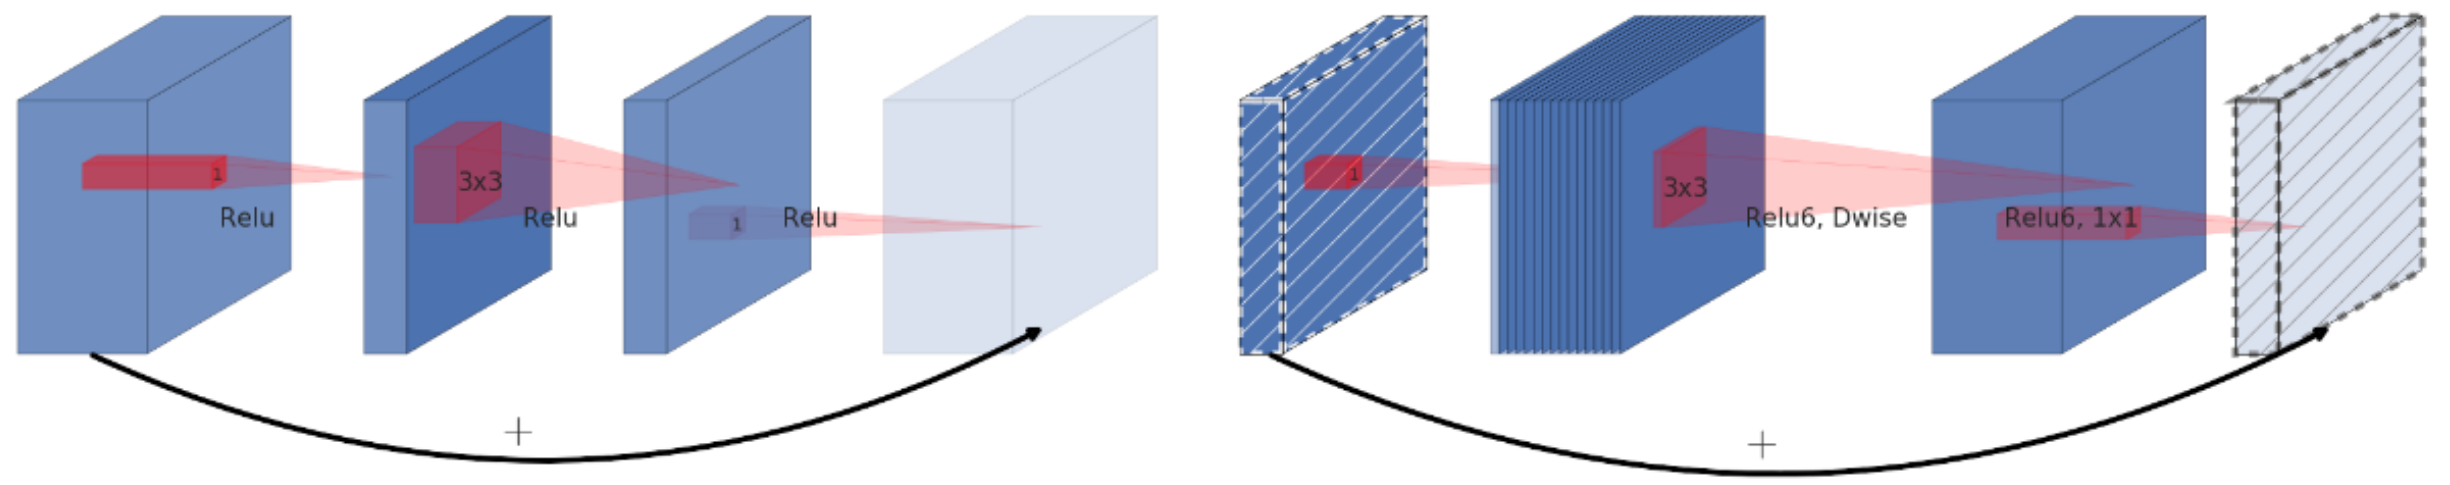
\includegraphics[scale=0.16]{mobilenet.png}
    \caption{Comparison between ResNet's residual block (left)~\autocite{chenMobileFaceNetsEfficientCNNs2018} with the inverted residual block proposed by MobileNetV2 (right)~\autocite{sandlerMobileNetV2InvertedResiduals2019} and used by MobileFaceNet. Image taken from MovileNetV2's paper~\autocite{sandlerMobileNetV2InvertedResiduals2019}.}
    \label{fig:mobilefacenet}
\end{figure}

\phantomsection\label{mobilefacenet}
\noindent\textbf{$\rightarrow$ MobileFaceNet}~\autocite{chenMobileFaceNetsEfficientCNNs2018} is a set of face verification CNN models designed to perform in real time and with high accuracy on mobile and embedded devices. It is built upon the inverted residual bottlenecks \reffig{fig:mobilefacenet} proposed in the general architecture lightweight CNN MobileNetV2~\autocite{sandlerMobileNetV2InvertedResiduals2019} that have the purpose of reducing the number of parameters of the network. The general residual bottleneck block~\autocite{heDeepResidualLearning2016} is composed of an input, followed by bottlenecks to reduce dimension and finished with an expansion to restore it, and the shortcut connects the high dimension layers. On the other hand, in the inverted residual architecture, it is considered that the information is stored in the bottleneck layers and the expansion is a mere implementation detail, therefore, a shortcut is placed directly between the bottlenecks. To solve the accuracy problem of face recognition CNNs that have a global average pooling layer, MobileFaceNets replaces it by a global depthwise convolution layer with kernel of size 7x7x1280 followed by a 1x1 convolution as the feature output layer. The primary MobileFaceNet architecture has 0.99 million parameters, but there is also the MobileFaceNet-M (the final 1x1 convolution is removed) and the MobileFaceNet-S (the 1x1 linear convolution before the global depthwise convolution is also removed).

\vspace{0.7\baselineskip}
\begin{figure}[H]
    \centering
    \begin{subfigure}{\textwidth}
        \centering
        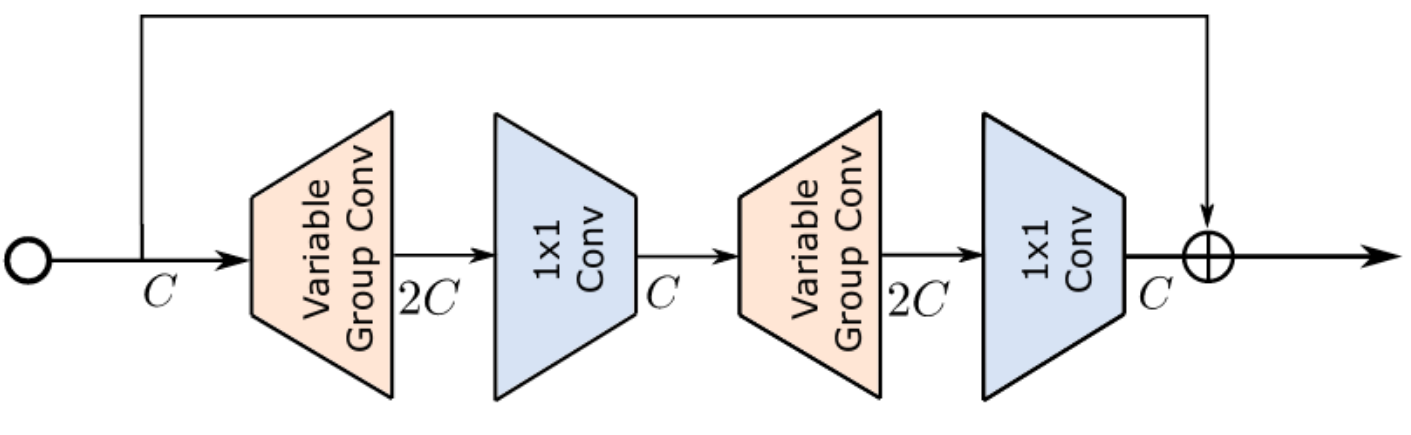
\includegraphics[scale=0.17]{vargnet_normal.png}
    \end{subfigure}
    
    \begin{subfigure}{\textwidth}
        \centering
        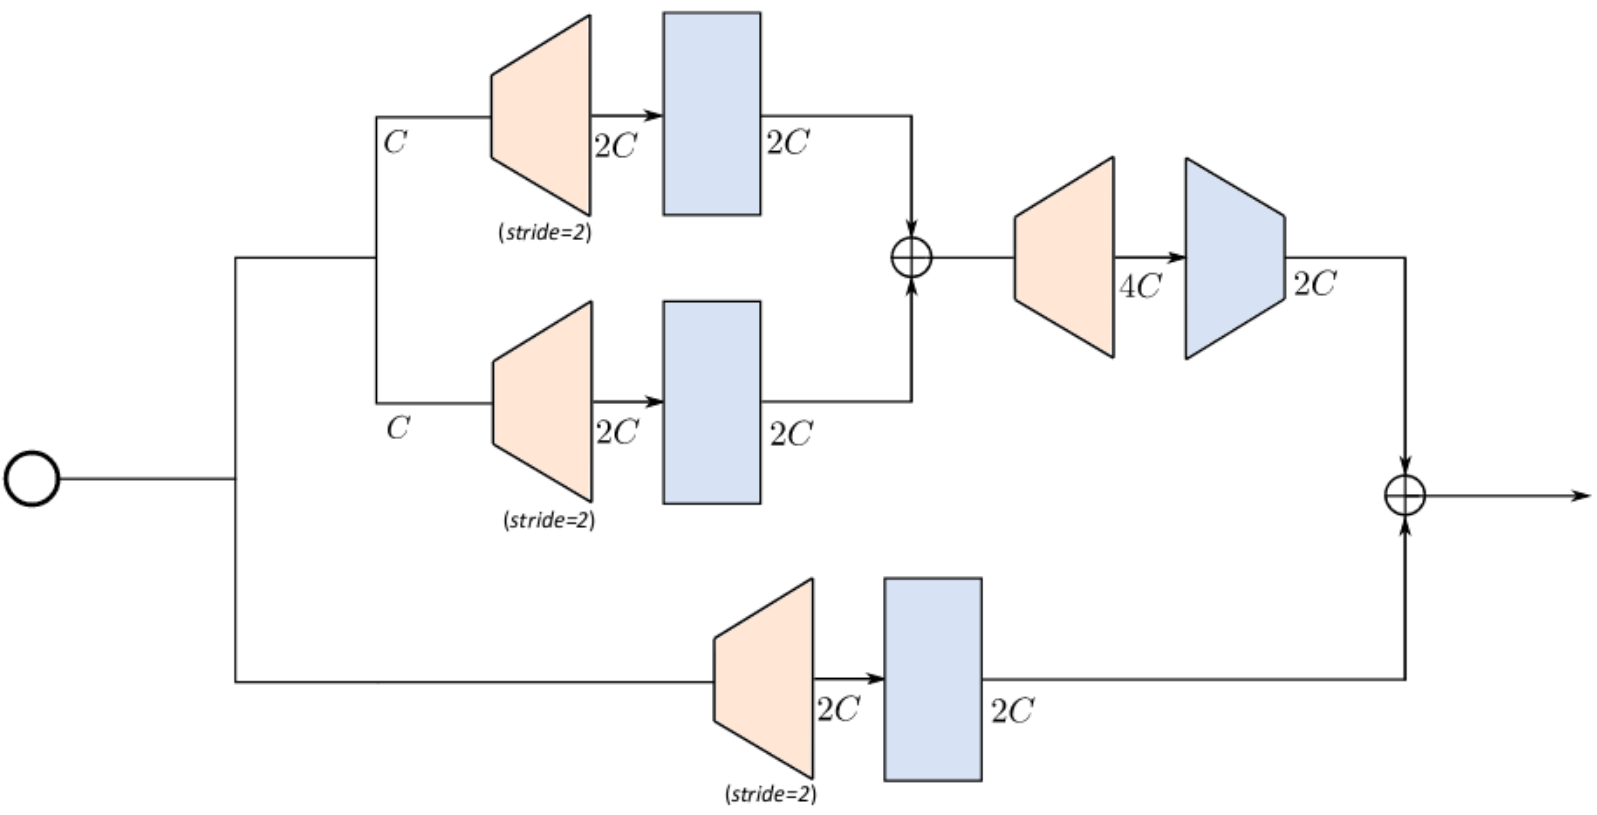
\includegraphics[scale=0.17]{vargnet_ds.png}
    \end{subfigure}
    
    \caption{VargNet's normal block (top) and downsampling block (bottom)~\autocite{zhangVarGNetVariableGroup2020} used by VargFaceNet. Image from VargNet's paper~\autocite{zhangVarGNetVariableGroup2020}.}
    \label{fig:vargnet}
\end{figure}

\noindent\textbf{$\rightarrow$ VarGFaceNet}~\autocite{yanVarGFaceNetEfficientVariable2019} is a lightweight face recognition CNN implementation based on the VarGNet architecture~\autocite{zhangVarGNetVariableGroup2020}~\autocite{chenMobileFaceNetsEfficientCNNs2018} that introduced a variable group convolution to solve unbalance of computational intensity due to hardware and compilers optimization. VarGFaceNet will use the normal and downsampling blocks from the VarGNet CNN \reffig{fig:vargnet}, but will add a Squeeze and Excitation (SE) block~\autocite{huSqueezeandExcitationNetworks2019} and replace the usual ReLU activation function by the PReLU~\autocite{heDelvingDeepRectifiers2015} one, since it is better for face recognition tasks. Other than that, the head setting is also changed without losing discriminative ability. The network is started with a 3x3 convolution with stride 1 that preserves the input size, instead of the downsampling 3x3 one with stride 2 from VarGNet. Finally, the embedding setting is also modified by performing variable group convolution and pointwise convolution to shrink the feature map to a 512-dimensional feature vector that is fed to the fully connected layer. In conclusion, the VarGFaceNet network is capable of performing accurate face recognition while maintaining a low amount of 5 million parameters.

\vspace{0.7\baselineskip}
\begin{figure}[H]
    \centering
    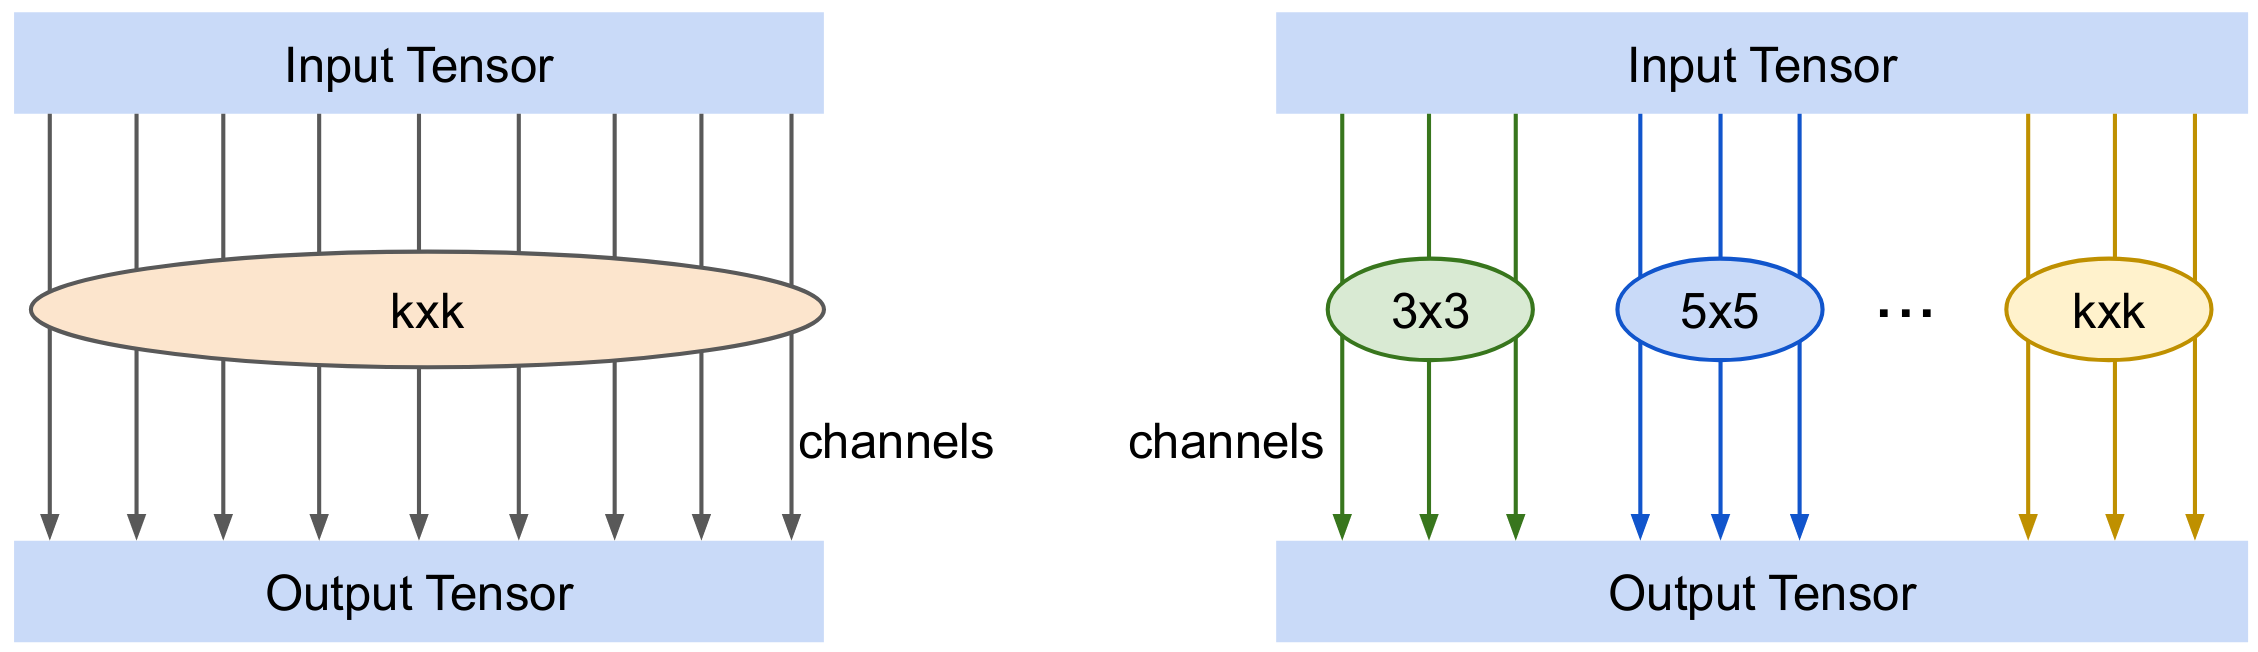
\includegraphics[scale=0.16]{mixconv.png}
    \caption{A normal convolution block that uses a single kernel (left) and the Mixed Depthwise Convolution proposed by MixNet~\autocite{tanMixConvMixedDepthwise}.}
    \label{fig:mixconv}
\end{figure}

\noindent\textbf{$\rightarrow$ MixFaceNet}~\autocite{boutrosMixFaceNetsExtremelyEfficient2021} is a lightweight implementation of MixNet~\autocite{tanMixConvMixedDepthwise} tailored for face verification. MixNet introduced Mixed Depthwise Convolution Kernels \reffig{fig:mixconv} that extends the theory behind depthwise convolution, but employs multiple kernel sizes in a single convolution, promoting the capturing of different patterns from distinct resolutions while reducing the number of parameters needed. The main differences proposed by the MixFaceNet design compared to MixNet resides in the head and embedding settings. For the network head set-up, fast downsampling in the first convolution layer with a 3x3 kernel and stride of 2, and PReLU~\autocite{heDelvingDeepRectifiers2015} activation function are used. Regarding the embedding settings, the global average pooling layer used by the MixNet architecture is replaced by a global depthwise convolution, in the same manner as the previously described \hyperref[mobilefacenet]{MobileFaceNet}.

\begin{figure}[H]
    \centering
    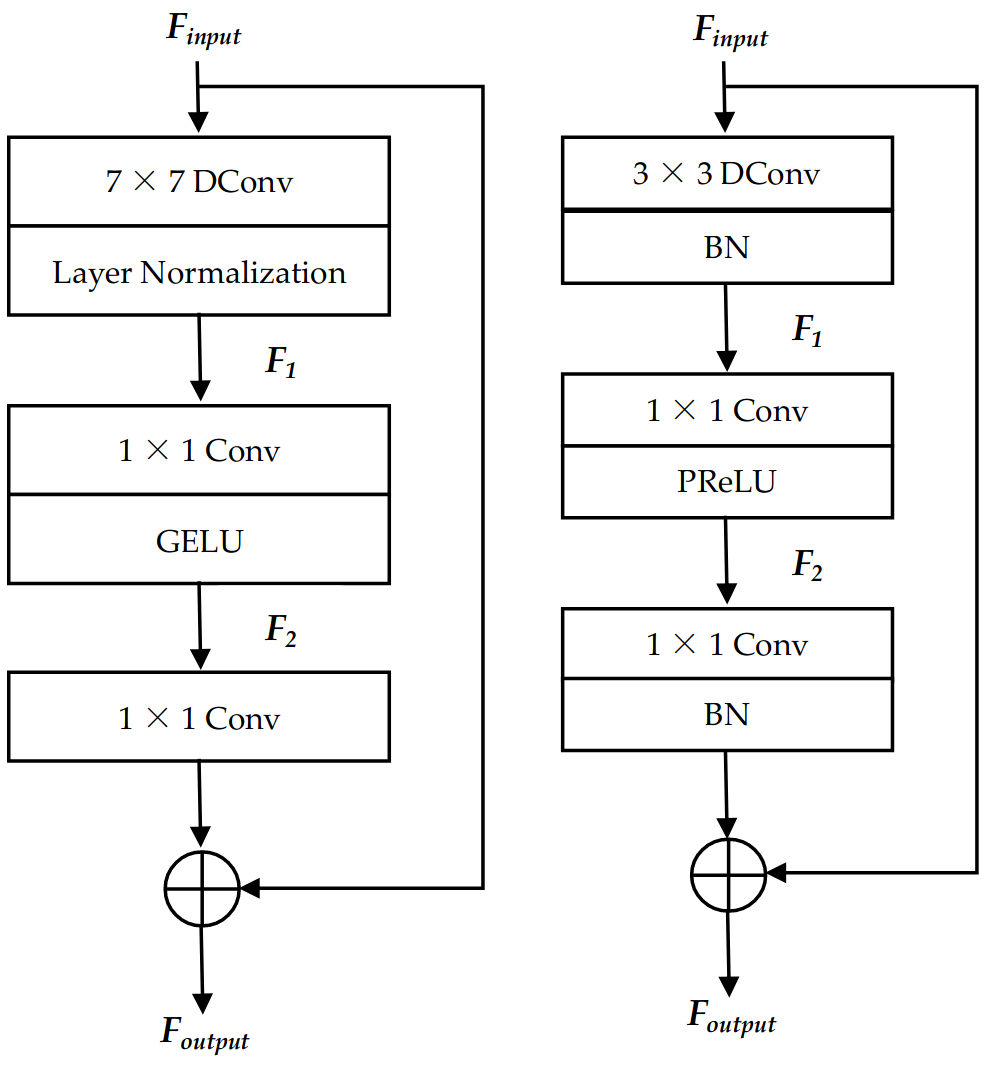
\includegraphics[scale=0.2]{convnext.png}
    \caption{Convolutional block proposed by ConvNeXt~\autocite{liuConvNet2020s2022} (top) and the one by ConvFaceNeXt~\autocite{hooConvFaceNeXtLightweightNetworks2022} (bottom). Image from the ConvFaceNeXt work~\autocite{hooConvFaceNeXtLightweightNetworks2022}.}
    \label{fig:convnext}
\end{figure}

\noindent\textbf{$\rightarrow$ ConvFaceNeXt}~\autocite{hooConvFaceNeXtLightweightNetworks2022} is a family of lightweight face recognition models, based on the ConvNeXt~\autocite{liuConvNet2020s2022} and MobileFaceNet architectures \reffig{fig:convnext}. The original ConvNeXt block is modified to better adapt to face recognition tasks and optimized to reduce the number of parameters. Accordingly, the Enhanced ConvNext (ECN) block is designed by adopting a smaller 3x3 kernel during the depthwise convolution, instead of the original 7x7 one. Adopting the principles studied in the MobileFaceNets implementation, rather than the usual layer of normalization and GeLU in the ConvNeXt model, batch normalization and PReLU~\autocite{heDelvingDeepRectifiers2015} are employed. 

\subsection{Loss}

\begin{figure}[!h]
    \centering
    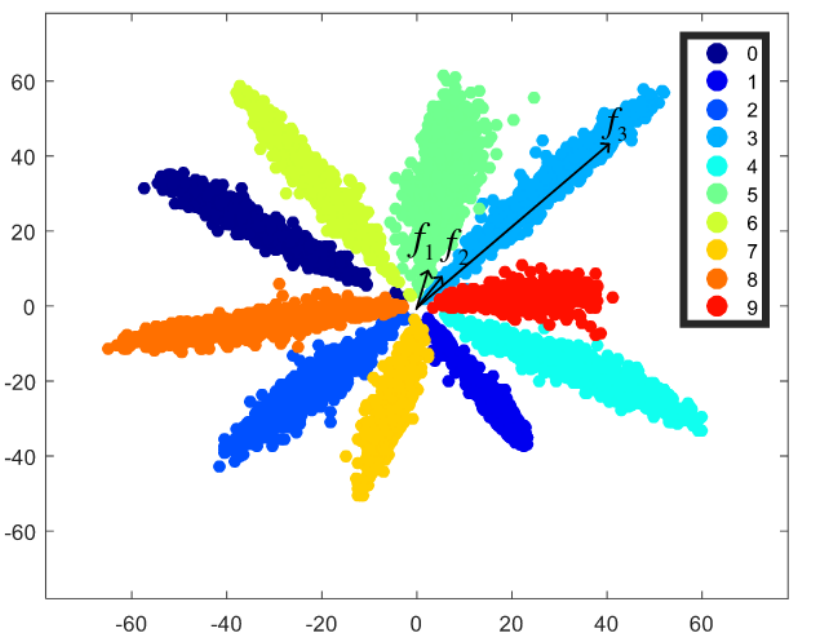
\includegraphics[scale=0.3]{compactness.png}
    \caption{Intra- and Inter-class challenge \autocite{wangNormFaceL2Hypersphere2017}. Eventhough features $f_2$ and $f_3$ belong to the same class, the euclidean distance between $f_1$ and $f_2$ is much smaller, proving the ineffectiveness of the softmax loss regarding inter-class compactness and inter-class separateness.}
    \label{fig:compactness}
\end{figure}

The initial face recognition proposals inherited principles from successful object classification implementations, henceforth, the most common loss function utilized was the well-known softmax loss. Unfortunately, it soon proved to be inefficient for face recognition applications since intra-variations (age gap between pictures of the same identity, for example) can be larger than inter-ones \reffig{fig:compactness}. Thus, the investigation interest shifted towards developing loss functions that had a better generalization ability and promoted more separable (to distinguish between an identity) and discriminative (to distinguish between identities) features~\autocite{wangDeepFaceRecognition2021}.
\par Face recognition can be achieved using either metric learning loss functions that learn a feature embedding to compute similarity or softmax-based loss functions that treat the problem as a classification task. Some works merge the two concepts.

\subsubsection{Classification-based loss functions}
Classification-based loss functions, derived from the general object classification task, aim at learn an N-way classification of all the classes, where each class relates to an identity composed of several faces~\autocite{duElementsEndtoendDeep2022}.
\par Because the methods are classification-based, the pioneers such as DeepFace or DeepID~\autocite{sunDeepLearningFace2014a}, utilized the most widely implemented loss function for classification, i.e. the softmax loss. It consists of a fully connected layer, the softmax function and cross-entropy loss, and can be formulated as follows:
\begin{equation}
\mathcal{L} = -\frac{1}{N}\sum_{i=1}^{N}\log{\frac{e^{W_{y_i}^{T}x_i+b_{y_i}}}{\sum_{j=1}^{c}e^{W_{j}^{T}x_i+b_{j}}}},
\end{equation}

\noindent where $N$ is the number of images, $c$ is the number of identities, $y_i$ is the $x_i$'s ground-truth label, $W_{y_i}$ is the ground-truth weight from $x_i$ in the fully connected layer and $b_j$ is a bias term. The term inside the logarithm represents the probability on the ground-truth class and the training objective is to maximize this probability.

\vspace{\baselineskip}
\par Taking the aforementioned principles and the drawbacks of lackluster generalization, and separable/discriminative abilities, the following loss functions proposed improving the softmax loss to better serve face recognition tasks.

\vspace{0.7\baselineskip}
\noindent\textbf{$\rightarrow$ NormFace}~\autocite{wangNormFaceL2Hypersphere2017} improves the classic softmax loss by studying the effect of $L_2$ normalization to the features and weights during the training stage. Because introducing this constraint resulted in the network not converging, a scale factor is also adopted that resizes the cosine similarity's scale between features and weights. This normalized softmax loss function can de reformulated as
\begin{equation}
\mathcal{L}_{norm} = -\frac{1}{N}\sum_{i=1}^{N}\log{\frac{e^{s \cos{(\theta_{y_i})}}}{e^{s \cos{(\theta_{y_i})}}+\sum_{j=1, j\neq y_i}^{c}s \cos{(\theta_{j})}}},
\end{equation}

\noindent where $s$ is the scale parameter and $\cos{(\theta_j)}$ results from the inner product between the $L_2$ normalized  weights $W_j$ and features $x_i$, i.e., $\cos{(\theta_j)}=\frac{\langle x_i, W_j\rangle}{\|W_j\|_2\|i_i\|_2}$

\begin{figure}[!h]
    \centering
    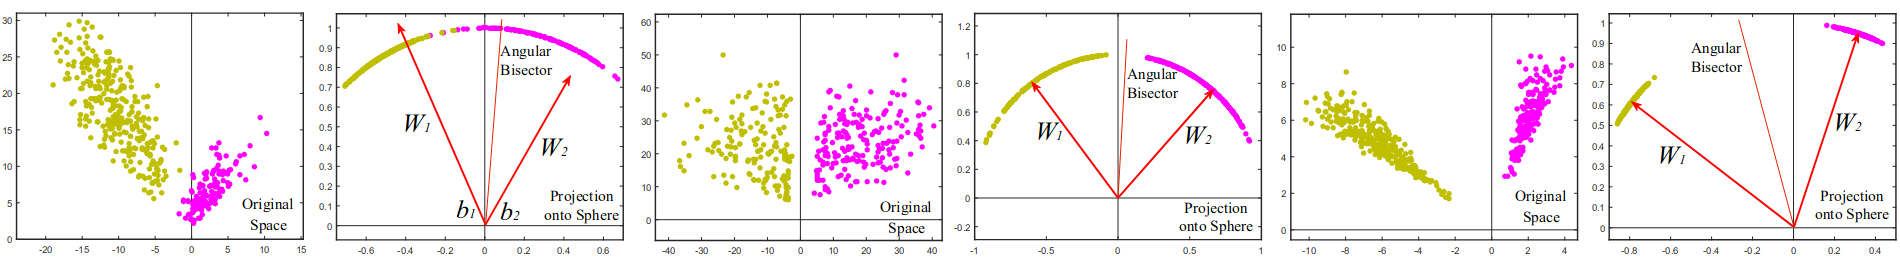
\includegraphics[scale=0.215]{sphereface.png}
    \caption{Comparison between the classic softmax loss, modified softmax loss (NormFace)~\autocite{wangNormFaceL2Hypersphere2017} and SphereFace \autocite{liuSphereFaceDeepHypersphere2018}.}
    \label{fig:sphereface}
\end{figure}

\vspace{0.7\baselineskip}
\noindent\textbf{$\rightarrow$ SphereFace}~\autocite{liuSphereFaceDeepHypersphere2018} improved the intra-class compactness and inter-class distance by introducing a very important concept of angular margin that contrasts with the usual Euclidean margin. As proven by Liu \textit{et al.}, features learned by softmax loss adopt an intrinsic angular distribution, therefore, euclidean margins are not compatible with softmax loss \reffig{fig:sphereface}. The decision boundary for a classic softmax loss function is $(W_1 - W_2)x+b_1-b_2=0$, and by normalizing the weights and zeroing the bias, it becomes $\|x\|(\cos{(\theta_1)}-\cos{(\theta_2)})=0$, where $x$ is a feature vector and the decision will only depend on the angles between class 1 and 2. SphereFace introduces the hyperparameter $m$ ($m\geq1 \in \mathbb{Z}$) that will, effectively, control the margin size between class 1 and 2 respectively as such $\|x\|(\cos{(m\theta_1)}-\cos{(\theta_2)})=0$ and $\|x\|(\cos{(\theta_1)}-\cos{(m\theta_2)})=0$.


\vspace{0.7\baselineskip}
\noindent\textbf{$\rightarrow$ AM-Softmax} and \textbf{CosFace} both improved SphereFace's main problem: the potential unstable training convergence due to the multiplicative angular margin. Thus, an additive cosine margin $\cos{\theta_{y_i}}+m$ is proposed to facilitate the convergence.

\begin{figure}[H]
    \centering
    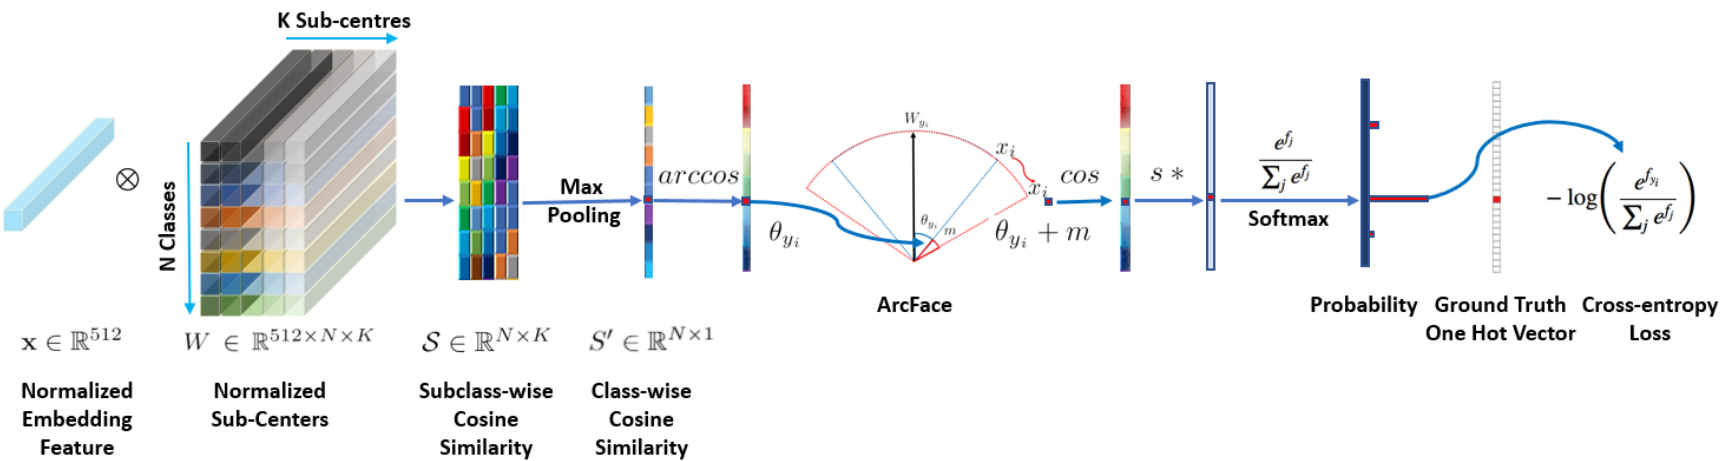
\includegraphics[scale=0.215]{arcface.png}
    \caption{ArcFace training process as described in the original paper~\autocite{dengArcFaceAdditiveAngular}.}
    \label{fig:arcface}
\end{figure}

\noindent\textbf{$\rightarrow$ ArcFace}~\autocite{dengArcFaceAdditiveAngular} aims at optimizing the geodesic distance margin since there is a mathematical correspondence between the angle and the arc in the normalized hypersphere. The concept behind this is described in \reffig{fig:arcface}. First, the cosine distance among features is obtained by the dot product between the feature produced by the CNN and the fully connected layer. After that, the arc-cosine is used to calculate the angle between the feature and the target one. Finally, the authors took the principles from AM-softmax \autocite{wangAdditiveMarginSoftmax2018} and SphereFace \autocite{liuSphereFaceDeepHypersphere2018}, and introduced an additive angular margin directly to the angle $\cos{(\theta_{y_i}+m)}$, getting the target logit back by the cosine function and further stabilizing the training process and improving the discriminative power of the overall system. The loss function is reformulated by: 1) zeroing the bias and transforming the softmax loss logit $W^{T}_{j}x_i=\|W_j\|x_i\|\cos{(\theta_j)}$, as suggested in~\autocite{liuSphereFaceDeepHypersphere2018}, where $\theta_j$ is the angle between the weight $W_J$ and the feature $x_i$, 2) following~\autocite{wangNormFaceL2Hypersphere2017,liuSphereFaceDeepHypersphere2018,wangCosFaceLargeMargin2018} the weights are normalized by $L_2$, 3) the features $x$ are also normalized in $L_2$ per~\autocite{ranjanL2constrainedSoftmaxLoss2017,wangNormFaceL2Hypersphere2017,wangAdditiveMarginSoftmax2018,wangCosFaceLargeMargin2018} suggestion. This normalization insures that there is only an angular dependence between weights and features, and the learned features are distributed along a hypersphere with radius $s$. To conclude, ArcFace can be described as follos:
\begin{equation}
\mathcal{L}=-\log\left(
                \frac{e^{s(\cos{(\theta_{y_i}+m)})}}
                {e^{s(\cos{(\theta_{y_i}+m)})} + \sum_{j=1, j\neq y_i}^{N}e^{s \cos{(\theta_j)}}}
            \right),
\end{equation}
\noindent where $m$ is the employed additive angular margin penalty between the feature $x_i$ and the ground truth center $W_{y_i}$ to promote the intra-class compactness and inter-class distance \reffig{fig:norm_arcface}.

\begin{figure}[H]
    \centering
    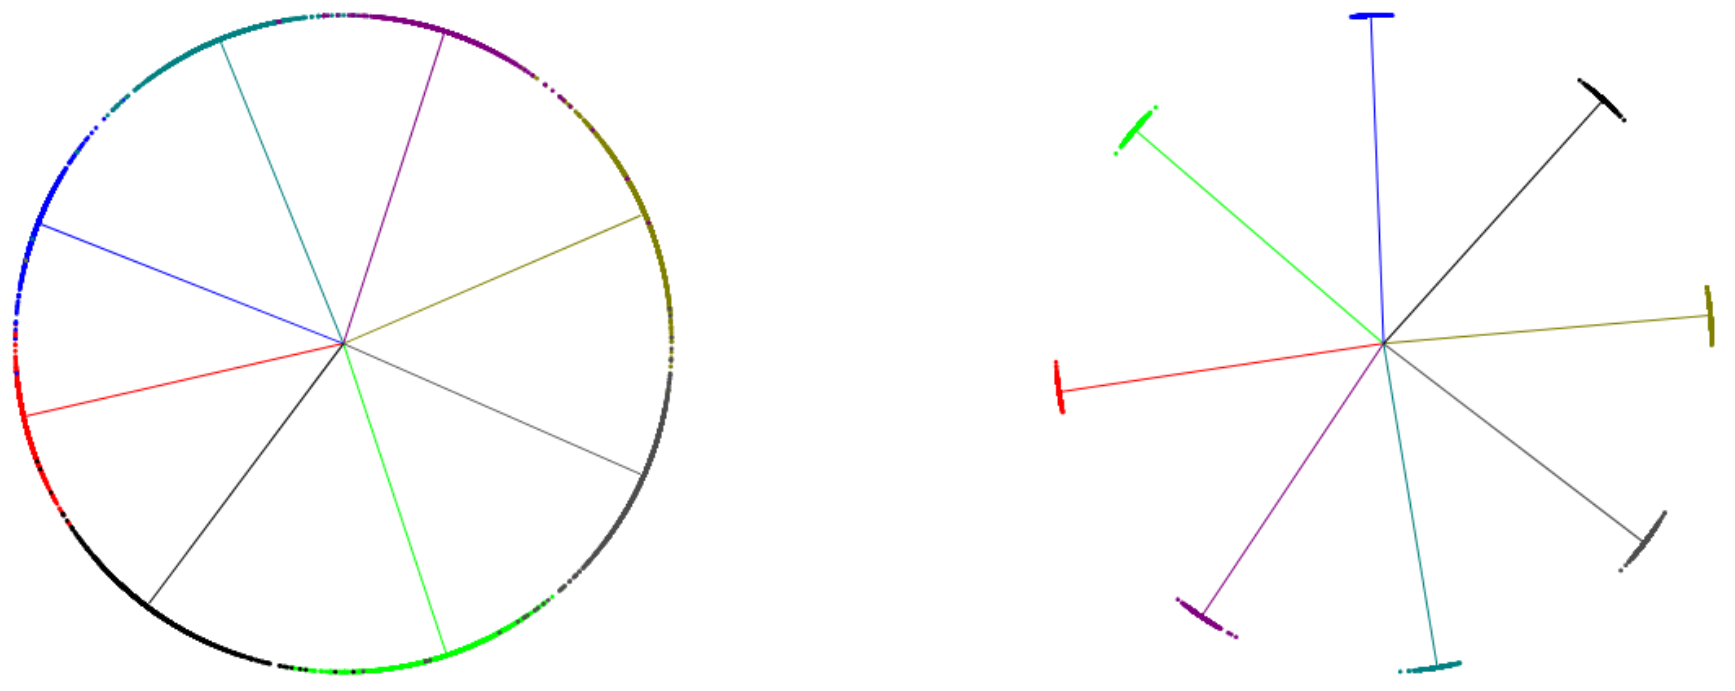
\includegraphics[scale=0.13]{norm_arc.png}
    \caption{Demonstration of the intra-class compactness and inter-class distance of ArcFace (right) compared to Norm-Softmax (left) for 8 identities. The distance margin between classes is clear for ArcFace. Image from ArcFace's paper ~\autocite{dengArcFaceAdditiveAngular}.}
    \label{fig:norm_arcface}
\end{figure}

\par To this day, ArcFace is still the state-of-the-art regarding face recognition, and one of the most implemented loss functions of this category, and it is usual to see other novel losses to use it as a starting point. The accuracy saturation of more common benchmarks like LFW~\autocite{huangLabeledFacesWild} lead to the appearance of harder ones, which will lead to loss functions aimed at more specific challenges, namely CurricularFace~\autocite{huangCurricularFaceAdaptiveCurriculum2020}, MagFace~\autocite{mengMagFaceUniversalRepresentation2021}, AdaFace~\autocite{kimAdaFaceQualityAdaptive2022} or QMagFace~\autocite{terhorstQMagFaceSimpleAccurate2023}.

\subsubsection{Metric learning loss functions}
Metric learning loss functions include the methods that aim optimizing the distance between feature embeddings. That is, increase the distance between negative embeddings and minimize the distance for those that are positive.
\par One classic example is the contrastive loss, but this category's attention mainly pends over the triplet loss first implemented by Schroff \textit{et al.} in FaceNet~\autocite{schroffFaceNetUnifiedEmbedding2015}. 

\vspace{0.7\baselineskip}
\noindent\textbf{$\rightarrow$ Contrastive Loss}~\autocite{duElementsEndtoendDeep2022} has the objective of optimizing the distance between identity pairs: positive pairs are encouraged to be closer and negative ones to be further apart. The loss function to be minimized is

\begin{equation}
    \mathcal{L}_{contrastive} = 
    \begin{cases}
      \frac{1}{2}\|f(x_i)-f(x_j)\|^{2}_{2}, \text{if} y_i=y_j\\
      \frac{1}{2}\max{(0, m_d-\|f(x_i)-f(x_j)\|_2)^2}, \text{if} y_i\neq y_j
    \end{cases}
\end{equation}

\begin{figure}[!h]
    \centering
    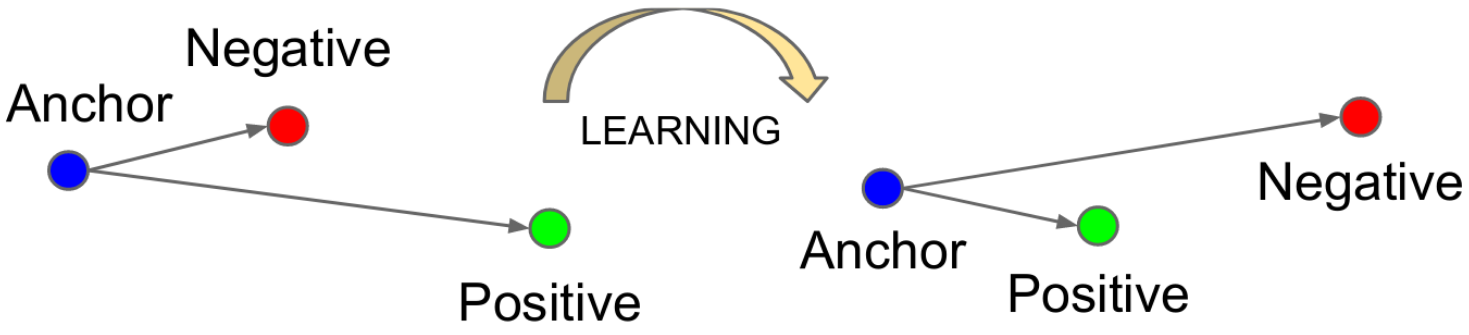
\includegraphics[scale=0.215]{triplet.png}
    \caption{Representation of training using triplet loss. Image from Facenet's paper \autocite{schroffFaceNetUnifiedEmbedding2015}.}
    \label{fig:triplet}
\end{figure}

\vspace{0.7\baselineskip}
\noindent\textbf{$\rightarrow$ Triplet Loss (2014)}~\autocite{schroffFaceNetUnifiedEmbedding2015} embeds an image to a d-dimensional feature vector in an Euclidean space. The motivation is to guarantee that, for every individual $i$, the squared distance between an image $x^{a}_{i}$ (anchor) of an identity and its corresponding true identities $x^{p}_{i}$ (positive) is smaller than the distance between non-identities, $x^{n}_{i}$ (negative). This structure is called a triplet \reffig{fig:triplet}. The aforesaid can be described in mathematical terms as:
\begin{equation}
\|f(x^{a}_{i})-f(x^{p}_{i})\|^{2}_{2} + \alpha < \|f(x^{a}_{i})-f(x^{n}_{i})\|^{2}_{2},
\end{equation}

\noindent where $f(\dot)$ are the feature embeddings from all the possible triplets, and $\alpha$ is a margin between positive and negative pairs. Therefore, the loss function to be optimized is:
\begin{equation}
\mathcal{L}_{triplet} = \sum_{i}^{N}\left[\|f(x^{a}_{i})-f(x^{p}_{i})\|^{2}_{2}-\|f(x^{a}_{i})-f(x^{n}_{i})\|^{2}_{2}+\alpha\right]
\end{equation}

\par However, there is a major drawback associated with this methodology. The selection of the triplets has a significant impact on the results and there is a combinatorial explosion regarding the number of possible triplets, specially for large-scale datasets, leading to a slower convergence and computational overhead if all the possible triplets are to be used. The only way to address this problem is through the development of efficient mining strategies that select both hard and representative triplets.

\section{Related work}
\label{sec:related_work}
The development of solutions for student monitoring, specially image-based, has encompassed a plethora of possibilities that can face several challenges, specially not being capable of controlling the capturing conditions or the computational power of the device where the system is executed. Depending on the application, they can be intended for commercial purposes or developed as part of academic research. Commercial solutions such as Kryterion, ProctorExam, ProctorU, Procotorio, ProctorFree, or SMOWL~\autocite{portugalContinuousUserIdentification2023} are available; however, with the exception of SMOWL, due to their proprietary nature, their methods of implementation are not disclosed, not allowing to study them adequately. Therefore, all the methods analyzed, except SMOWL, will fall under the second category.

\vspace{0.7\baselineskip}
\noindent\textbf{$\rightarrow$ Zhang \textit{et al.}~\autocite{zhangVirtualLaboratorySystem2016} (2016)} studied a system based on facial features exclusively. The faces are first detected and extracted using the OpenCV pretrained classifier based on the Viola-Jones/Haar Cascades algorithm. Subsequently, recognition is carried out utilizing the Eigenfaces algorithm, which incorporates Principal Component Analysis (PCA). The main disadvantage of this solution is lacking the flexibility to adverse visual conditions that Deep Learning techniques have.

\vspace{0.7\baselineskip}
\noindent\textbf{$\rightarrow$ Atoum \textit{et al.}~\autocite{atoumAutomatedOnlineExam2017} (2017)} proposed a solution that employs Viola-Jones/Haar Cascades face detector and Minimum Average Correlation Energy (MACE) filter for face verification. Once again, the methodologies utilized are too sensitive to image variations, such as illumination, pose, expressions, etc.

\vspace{0.7\baselineskip}
\noindent\textbf{$\rightarrow$ Zhang \textit{et al.}~\autocite{zhangVirtualProctorBiometric2018} (2018)} latter proposed another solution. In a similar fashion to Zhang \textit{et al.}~\autocite{zhangVirtualLaboratorySystem2016} and Atoum \textit{et al.}~\autocite{atoumAutomatedOnlineExam2017}, the face detection is achieved through the same OpenCV pretrained module. On the other hand, the detected and cropped faces are now processed by a modification of the Stereo Matching algorithm. Because this method extracts information from pairs of stereo images, it is subject to occlusions, ambiguities, textures, etc.

\vspace{0.7\baselineskip}
\noindent\textbf{$\rightarrow$ Sawhney \textit{et al.}~\autocite{sawhneyRealTimeSmartAttendance2019} (2019)} introduced an approach where the face detection is accomplished in two stages: 1) bounding box regression with the Viola-Jones/Haar Cascades algorithm and 2) facial landmark generation with a Local Model-based algorithm. After the faces are extracted, the face recognition stage, in similarity with Zhang \textit{et al.}~\autocite{zhangVirtualLaboratorySystem2016}, applies simultaneously Eigenfaces with PCA, therefore, the drawbacks coincide.


\vspace{0.7\baselineskip}
\noindent\textbf{$\rightarrow$ Ganidisastra and Bandung~\autocite{ganidisastraIncrementalTrainingDeep2021} (2021)} introduced a Deep Learning-based approach that employs two models for face detection and recognition: YOLO-face for face detection and Facenet for face recognition. Notably, Facenet is continuously trained with data collected at the end of each user session. This training process causes the system to overfit to each individual identity, leading to reduced adaptability in handling new scenarios due to limited data availability. Furthermore, the training of Facenet utilizes the triplet loss, which can be computationally challenging, especially on less powerful hardware. This is primarily due to the exponential increase in possible combinations when mining triplets during the training process.

\vspace{0.7\baselineskip}
\noindent\textbf{$\rightarrow$ SMOWL~\autocite{labayenOnlineStudentAuthentication2021} (2021)} is a multi-modal tool that analyzes voice, face and key-strokes data. For this dissertation, the interest resides only on the facial aspect of it. For face detection, it utilizes a combination of FaceBoxes with MobileNet-SSD for occlusion detection. The face recognition is accomplished with a Facenet model trained with triplet loss on the MS-Celeb-1M dataset. Anew, the triplet loss training can be considered a drawback. 

\vspace{0.7\baselineskip}
\noindent\textbf{$\rightarrow$ TrustID~\autocite{fariaImagebasedFaceVerification2023} (2023)} is our solution, designed and developed at ISR - UC. It utilizes as a face detection a linear detector conjointly with a Histogram of Oriented Gradients and pyramidal image search. After the faces are detected and aligned, they are cropped to a Region of Interest (RoI) of $150\times150$ pixels. Finally, the faces are passed to a face recognition module that uses a CNN with 29 layers based on the ResNet-34, trained with triplet loss on a dataset of, approximately, 3 million faces derived from the Visual Geometry Group
Face~\autocite{parkhiDeepFaceRecognition2015} and FaceScrub~\autocite{ngDatadrivenApproachCleaning2014} datasets.


\vspace{\baselineskip}
\par The primary focus of this work revolves around the selection of the architecture for the face recognition module, which, as previously mentioned, will exclusively center on image-based Deep Learning approaches. In pursuit of this goal, the monitoring system must proactively address potential, previously mentioned, challenges that may arise during data acquisition. Deep Learning methods have shown remarkable capabilities in tackling such challenges effectively.

\par In particular, the face recognition module must exhibit robustness in handling variations in illumination, pose, and image quality, especially in scenarios where precise control over these factors is unattainable. Furthermore, we need to consider the computational resources available to users, as students may access the system using smartphones or less powerful computing devices. Consequently, our choice of framework must be resilient to these variations and resource constraints.

\end{document}